
%% Package and Class "uiucthesis2014" for use with LaTeX2e.
\documentclass{report}

\usepackage[acronym,toc]{glossaries}
%\newacronym{<++>}{<++>}{<++>}
\newacronym[longplural={metric tons of heavy metal}]{MTHM}{MTHM}{metric ton of heavy metal}
\newacronym{ABM}{ABM}{agent-based modeling}
\newacronym{ACDIS}{ACDIS}{Program in Arms Control \& Domestic and International Security}
\newacronym{ADS}{ADS}{Accelerator-Driven Systems}
\newacronym{AHTR}{AHTR}{Advanced High Temperature Reactor}
\newacronym{ANDRA}{ANDRA}{Agence Nationale pour la gestion des D\'echets RAdioactifs, the French National Agency for Radioactive Waste Management}
\newacronym{ANL}{ANL}{Argonne National Laboratory}
\newacronym{ANS}{ANS}{American Nuclear Society}
\newacronym{API}{API}{application programming interface}
\newacronym{ARE}{ARE}{Aircraft Reactor Experiment}
\newacronym{ARFC}{ARFC}{Advanced Reactors and Fuel Cycles}
\newacronym{ASME}{ASME}{American Society of Mechanical Engineers}
\newacronym{ASTRID}{ASTRID}{Advanced Sodium Technological Reactor for Industrial Demonstration}
\newacronym{ATWS}{ATWS}{Anticipated Transient Without Scram}
\newacronym{BDBE}{BDBE}{Beyond Design Basis Event}
\newacronym{BIDS}{BIDS}{Berkeley Institute for Data Science}
\newacronym{BWR}{BWR}{Boiling Water Reactor}
\newacronym{CAFCA}{CAFCA}{ Code for Advanced Fuel Cycles Assessment }
\newacronym{CANDU}{CANDU}{Canada Deuterium Uranium}
\newacronym{CDTN}{CDTN}{Centro de Desenvolvimento da Tecnologia Nuclear}
\newacronym{CEA}{CEA}{Commissariat \`a l'\'Energie Atomique et aux \'Energies Alternatives}
\newacronym{CI}{CI}{continuous integration}
\newacronym{CNEN}{CNEN}{Comiss\~{a}o Nacional de Energia Nuclear}
\newacronym{CNERG}{CNERG}{Computational Nuclear Engineering Research Group}
\newacronym{CORRM}{CORRM}{Continuous On-Line Reprocessing Reactor Module}
\newacronym{COSI}{COSI}{Commelini-Sicard}
\newacronym{COTS}{COTS}{commercial, off-the-shelf}
\newacronym{CSNF}{CSNF}{commercial spent nuclear fuel}
\newacronym{CTAH}{CTAHs}{Coiled Tube Air Heaters}
\newacronym{CUBIT}{CUBIT}{CUBIT Geometry and Mesh Generation Toolkit}
\newacronym{CURIE}{CURIE}{Centralized Used Fuel Resource for Information Exchange}
\newacronym{DAG}{DAG}{directed acyclic graph}
\newacronym{DANESS}{DANESS}{Dynamic Analysis of Nuclear Energy System Strategies}
\newacronym{DBE}{DBE}{Design Basis Event}
\newacronym{DESAE}{DESAE}{Dynamic Analysis of Nuclear Energy Systems Strategies}
\newacronym{DHS}{DHS}{Department of Homeland Security}
\newacronym{DOE}{DOE}{Department of Energy}
\newacronym{DU}{DU}{depleted uranium}
\newacronym{DRACS}{DRACS}{Direct Reactor Auxiliary Cooling System}
\newacronym{DRE}{DRE}{dynamic resource exchange}
\newacronym{DSNF}{DSNF}{DOE spent nuclear fuel}
\newacronym{DYMOND}{DYMOND}{Dynamic Model of Nuclear Development }
\newacronym{EBS}{EBS}{Engineered Barrier System}
\newacronym{EDF}{EDF}{Électricité de France}
\newacronym{EFPD}{EFPD}{Effective Full Power Days}
\newacronym{EDS}{EDS}{Externally Driven Systems}
\newacronym{EDZ}{EDZ}{Excavation Disturbed Zone}
\newacronym{EIA}{EIA}{U.S. Energy Information Administration}
\newacronym{EPA}{EPA}{Environmental Protection Agency}
\newacronym{EPR}{EPR}{European Pressurized Reactor}
\newacronym{EP}{EP}{Engineering Physics}
\newacronym{EU}{EU}{European Union}
\newacronym{FCO}{FCO}{Fuel Cycle Options}
\newacronym{FCT}{FCT}{Fuel Cycle Technology}
\newacronym{FEHM}{FEHM}{Finite Element Heat and Mass Transfer}
\newacronym{FEPs}{FEPs}{Features, Events, and Processes}
\newacronym{FHR}{FHR}{Fluoride-Salt-Cooled High-Temperature Reactor}
\newacronym{FLiBe}{FLiBe}{Fluoride-Lithium-Beryllium}
\newacronym{FP}{FP}{Fission Product}
\newacronym{GDSE}{GDSE}{Generic Disposal System Environment}
\newacronym{GDSM}{GDSM}{Generic Disposal System Model}
\newacronym{GENIUSv1}{GENIUSv1}{Global Evaluation of Nuclear Infrastructure Utilization Scenarios, Version 1}
\newacronym{GENIUSv2}{GENIUSv2}{Global Evaluation of Nuclear Infrastructure Utilization Scenarios, Version 2}
\newacronym{GENIUS}{GENIUS}{Global Evaluation of Nuclear Infrastructure Utilization Scenarios}
\newacronym{GPAM}{GPAM}{Generic Performance Assessment Model}
\newacronym{GRSAC}{GRSAC}{Graphite Reactor Severe Accident Code}
\newacronym{GUI}{GUI}{graphical user interface}
\newacronym{HEU}{HEU}{high enriched uranium}
\newacronym{HLW}{HLW}{high level waste}
\newacronym{HPC}{HPC}{high-performance computing}
\newacronym{HTC}{HTC}{high-throughput computing}
\newacronym{HWR}{HWR}{Heavy Water Reactor}
\newacronym{HTGR}{HTGR}{High Temperature Gas-Cooled Reactor}
\newacronym{IAEA}{IAEA}{International Atomic Energy Agency}
\newacronym{IEA}{IEA}{International Energy Agency}
\newacronym{IEMA}{IEMA}{Illinois Emergency Mangament Agency}
\newacronym{IHLRWM}{IHLRWM}{International High Level Radioactive Waste Management}
\newacronym{INL}{INL}{Idaho National Laboratory}
\newacronym{IPRR1}{IRP-R1}{Instituto de Pesquisas Radioativas Reator 1}
\newacronym{IRP}{IRP}{Integrated Research Project}
\newacronym{ISFSI}{ISFSI}{Independent Spent Fuel Storage Installation}
\newacronym{ISRG}{ISRG}{Independent Student Research Group}
\newacronym{JFNK}{JFNK}{Jacobian-Free Newton Krylov}
\newacronym{LANL}{LANL}{Los Alamos National Laboratory}
\newacronym{LBNL}{LBNL}{Lawrence Berkeley National Laboratory}
\newacronym{LCOE}{LCOE}{levelized cost of electricity}
\newacronym{LDRD}{LDRD}{laboratory directed research and development}
\newacronym{LFR}{LFR}{Lead-Cooled Fast Reactor}
\newacronym{LLNL}{LLNL}{Lawrence Livermore National Laboratory}
\newacronym{LLW}{LLW}{Low Level Waste}
\newacronym{LMFBR}{LMFBR}{Liquid Metal Fast Breeder Reactor}
\newacronym{LOFC}{LOFC}{Loss of Forced Cooling}
\newacronym{LOHS}{LOHS}{Loss of Heat Sink}
\newacronym{LOLA}{LOLA}{Loss of Large Area}
\newacronym{LP}{LP}{linear program}
\newacronym{LWR}{LWR}{Light Water Reactor}
\newacronym{MAGNOX}{MAGNOX}{Magnesium Alloy Graphie Moderated Gas Cooled Uranium Oxide Reactor}
\newacronym{MA}{MA}{minor actinide}
\newacronym{MCNP}{MCNP}{Monte Carlo N-Particle code}
\newacronym{MCSFR}{MCSFR}{Molten Chloride Salt Fast Reactor}
\newacronym{MILP}{MILP}{mixed-integer linear program}
\newacronym{MIT}{MIT}{the Massachusetts Institute of Technology}
\newacronym{MOAB}{MOAB}{Mesh-Oriented datABase}
\newacronym{MOOSE}{MOOSE}{Multiphysics Object-Oriented Simulation Environment}
\newacronym{MOX}{MOX}{Mixed Oxide Fuel}
\newacronym{MSBR}{MSBR}{Molten Salt Breeder Reactor}
\newacronym{MSRE}{MSRE}{Molten Salt Reactor Experiment}
\newacronym{MSR}{MSR}{Molten Salt Reactor}
\newacronym{MWe}{MWe}{Megawatt Electric}
\newacronym{NAGRA}{NAGRA}{National Cooperative for the Disposal of Radioactive Waste}
\newacronym{NEAMS}{NEAMS}{Nuclear Engineering Advanced Modeling and Simulation}
\newacronym{NEUP}{NEUP}{Nuclear Energy University Programs}
\newacronym{NFC}{NFC}{nuclear fuel cycle}
\newacronym{NFCS}{NFC simulator}{nuclear fuel cycle simulator}
\newacronym{NGNP}{NGNP}{Next Generation Nuclear Plant}
\newacronym{NMWPC}{NMWPC}{Nuclear MW Per Capita}
\newacronym{NNSA}{NNSA}{National Nuclear Security Administration}
\newacronym{NPRE}{NPRE}{Department of Nuclear, Plasma, and Radiological Engineering}
\newacronym{NQA1}{NQA-1}{Nuclear Quality Assurance - 1}
\newacronym{NRC}{NRC}{Nuclear Regulatory Commission}
\newacronym{NSF}{NSF}{National Science Foundation}
\newacronym{NSSC}{NSSC}{Nuclear Science and Security Consortium}
\newacronym{NUWASTE}{NUWASTE}{Nuclear Waste Assessment System for Technical Evaluation}
\newacronym{NWF}{NWF}{Nuclear Waste Fund}
\newacronym{NWTRB}{NWTRB}{Nuclear Waste Technical Review Board}
\newacronym{OCRWM}{OCRWM}{Office of Civilian Radioactive Waste Management}
\newacronym{ORION}{ORION}{ORION}
\newacronym{ORNL}{ORNL}{Oak Ridge National Laboratory}
\newacronym{PARCS}{PARCS}{Purdue Advanced Reactor Core Simulator}
\newacronym{PBAHTR}{PB-AHTR}{Pebble Bed Advanced High Temperature Reactor}
\newacronym{PBFHR}{PB-FHR}{Pebble-Bed Fluoride-Salt-Cooled High-Temperature Reactor}
\newacronym{PEI}{PEI}{Peak Environmental Impact}
\newacronym{PH}{PRONGHORN}{PRONGHORN}
\newacronym{PHWR}{PHWR}{Pressurized Heavy Water Reactor}
\newacronym{PRIS}{PRIS}{Power Reactor Information System}
\newacronym{PRKE}{PRKE}{Point Reactor Kinetics Equations}
\newacronym{PSPG}{PSPG}{Pressure-Stabilizing/Petrov-Galerkin}
\newacronym{PWAR}{PWAR}{Pratt and Whitney Aircraft Reactor}
\newacronym{PWR}{PWR}{Pressurized Water Reactor}
\newacronym{PyNE}{PyNE}{Python toolkit for Nuclear Engineering}
\newacronym{PyRK}{PyRK}{Python for Reactor Kinetics}
\newacronym{QA}{QA}{quality assurance}
\newacronym{RDD}{RD\&D}{Research Development and Demonstration}
\newacronym{RD}{R\&D}{Research and Development}
\newacronym{RELAP}{RELAP}{Reactor Excursion and Leak Analysis Program}
\newacronym{RIA}{RIA}{Reactivity Insertion Accident}
\newacronym{RIF}{RIF}{Region-Institution-Facility}
\newacronym{RU}{RU}{reprocessed uranium}
\newacronym{ROM}{ROM}{Reduced Order Model}
\newacronym{SFR}{SFR}{Sodium-Cooled Fast Reactor}
\newacronym{SINDAG}{SINDA{\textbackslash}G}{Systems Improved Numerical Differencing Analyzer $\backslash$ Gaski}
\newacronym{SKB}{SKB}{Svensk K\"{a}rnbr\"{a}nslehantering AB}
\newacronym{SNF}{SNF}{spent nuclear fuel}
\newacronym{SNL}{SNL}{Sandia National Laboratory}
\newacronym{STC}{STC}{specific temperature change}
\newacronym{SUPG}{SUPG}{Streamline-Upwind/Petrov-Galerkin}
\newacronym{SWF}{SWF}{Separations and Waste Forms}
\newacronym{SWU}{SWU}{Separative Work Unit}
\newacronym{TRIGA}{TRIGA}{Training Research Isotope General Atomic}
\newacronym{TRISO}{TRISO}{Tristructural Isotropic}
\newacronym{TRU}{TRU}{transuranic}
\newacronym{TSM}{TSM}{Total System Model}
\newacronym{TSPA}{TSPA}{Total System Performance Assessment for the Yucca Mountain License Application}
\newacronym{ThOX}{ThOX}{thorium oxide}
\newacronym{UDB}{UDB}{Unified Database}
\newacronym{UFD}{UFD}{Used Fuel Disposition}
\newacronym{UML}{UML}{Unified Modeling Language}
\newacronym{UNF}{UNF}{Used Nuclear Fuel}
\newacronym{UNF-STANDARDS}{UNF-ST\&DARDS}{Used Nuclear Fuel Storage Transportation and Disposal Analysis Resource and Data System}
\newacronym{UOX}{UOX}{Uranium Oxide Fuel}
\newacronym{UQ}{UQ}{uncertainty quantification}
\newacronym{US}{US}{United States}
\newacronym{UW}{UW}{University of Wisconsin}
\newacronym{VISION}{VISION}{the Verifiable Fuel Cycle Simulation Model}
\newacronym{VVER}{VVER}{Voda-Vodyanoi Energetichesky Reaktor (Russian Pressurized Water Reactor)}
\newacronym{VV}{V\&V}{verification and validation}
\newacronym{WIPP}{WIPP}{Waste Isolation Pilot Plant}
\newacronym{YMR}{YMR}{Yucca Mountain Repository Site}

\usepackage{placeins}
\usepackage{booktabs} % nice rules (thick lines) for tables
\usepackage{microtype} % improves typography for PDF
\usepackage{xspace}
\usepackage[hidelinks]{hyperref}
\usepackage{xspace}
\usepackage{setspace}
\usepackage{hhline}
\usepackage{amsmath}
\usepackage{color}
\usepackage{multirow}
\usepackage{fourier}
\usepackage{booktabs}
\newcommand\tab[1][1cm]{\hspace*{#1}}

\usepackage{threeparttable, tablefootnote}

%tikzpicture fit to page width
\usepackage{environ}
\makeatletter
\newsavebox{\measure@tikzpicture}
\NewEnviron{scaletikzpicturetowidth}[1]{%
  \def\tikz@width{#1}%
  \def\tikzscale{1}\begin{lrbox}{\measure@tikzpicture}%
  \BODY
  \end{lrbox}%
  \pgfmathparse{#1/\wd\measure@tikzpicture}%
  \edef\tikzscale{\pgfmathresult}%
  \BODY
}

\usepackage{tabularx}
\newcolumntype{b}{>{\hsize=1.0\hsize}X}
\newcolumntype{s}{>{\hsize=.5\hsize}X}
\newcolumntype{m}{>{\hsize=.75\hsize}X}
\usepackage{graphics}
\newcommand{\Cycamore}{\textsc{Cycamore}\xspace}%
\newcommand{\Cyclus}{\textsc{Cyclus}\xspace}%
\newcommand{\uthree}{\xspace $^{233}_{92}U$ \xspace}
\newcommand{\ufive}{\xspace $^{235}_{92}U$\xspace}%%
\newcommand{\utwo}{\xspace $^{232}_{92}U$\xspace}
\newcommand{\ueight}{\xspace $^{238}_{92}U$\xspace}
\newcommand{\pu}{\xspace$^{239}_{94}Pu$\xspace}
\newcommand{\thor}{\xspace $^{232}_{90}Th$\xspace}
\graphicspath{ {images/} }
\usepackage[affil-it]{authblk}
\usepackage[numbers]{natbib}
\usepackage{notoccite}
\usepackage{tikz}
\usetikzlibrary{positioning, arrows, decorations, shapes}

\usetikzlibrary{shapes.geometric,arrows}
\tikzstyle{process} = [rectangle, rounded corners, minimum width=2.5cm, minimum height=1cm,text centered, draw=black, fill=blue!30]
\tikzstyle{object} = [ellipse, rounded corners, minimum width=3cm, minimum height=1cm,text centered, draw=black, fill=green!30]
\tikzstyle{empty} =  [rectangle, rounded corners, minimum width=2.5cm, minimum height=0.7cm,text centered, draw=black, fill=white!30]
\tikzstyle{arrow} = [thick,->,>=stealth]
\usepackage{cleveref}
\usepackage{datatool}


\begin{document}

\title{Fuel cycle transition simulation capabilities in Cyclus}

\author{Jin Whan Bae}
%\department{Department of Nuclear, Plasma, Radiological Engineering}
%\schools{B.S., University of Illinois - Urbana Champaign, 2017}
%\msthesis
%\advisor{Kathryn Huff}
%\degreeyear{2018}
%\committee{Professor Rizwan Uddin \\ Professor Clifford Singer}
\maketitle


%% Create an abstract that can also be used for the ProQuest abstract.
%% Note that ProQuest truncates their abstracts at 350 words.
\begin{abstract}

Recent interest in advanced reactors and the following need for techno-economic
transitions has increased the demand for tools necessary
to model complex \glspl{NFC} and advanced reactor technologies.
This thesis demonstrates the capability of Cyclus, the
agent-based fuel cycle simulator, to model, simulate, and analyze
real-life fuel cycle transition scenarios. I introduce new methods
and tools that use various databases to model and simulate real-world
nuclear fuel cycle transition scenarios involving advanced reactor
technologies.

The development of the capability takes
three steps: (1) benchmarking
Cyclus to other \glspl{NFCS};
(2) developing new methods and tools necessary for modeling and simulating
real-world fuel cycle transition scenarios; (3)
simulation of both domestic and international nuclear technology
transitions.

The methods and tools developed for such capabilities include:
(1) modeling and simulating past and current
nuclear fleets using historic nuclear reactor operations
database; (2) modeling individual reactors and its operating history
to calculate nuclear material inventory; (3) modeling \gls{MSR} behavior
in a large-scale fuel cycle simulation.

Benchmark work shows that Cyclus results coincide
with results from other \glspl{NFCS} with minor differences
due to modeling reactor behavior.
Additionally, this thesis demonstrates the Cyclus capability to effectively
model and simulate real-life \gls{NFC} transition scenarios
that involve advanced reactor technologies such as \glspl{MSR}.

\end{abstract}

\chapter*{Acknowledgments}


I consider all my output as a result of me standing on the shoulders
of giants. There have been multiple giants that were kind enough
to lend me their shoulders. Notably, the tallest of all, my advisor
and mentor Kathryn Huff, who patiently guided me from my academic
infancy. Also, I owe the world to my parents and loving brother who
brought me up with love
from my actual infancy.  I also thank the staff of Oak Ridge National Laboratory
Joushua L. Peterson-Droogh, Eva Davidson, Ben Betzler and Andrew Worrall for their
guidance over the summer.

I also cannot express enough gratitude to my friends and colleagues. My greatest
assets and partners that I have had the privilege to cohabitate with, Daniel
O'Grady and Steven Stemmley, who were the logical anchor in my life. Also, my colleagues
Andrei Rykhlevskii, Gwendolyn Chee, Gregory Westphal, Gyu Tae Park, Sun Myung Park, and
Anshuman Chuabe have been of great help. Last but not least I thank my long-time friends Jieon Kim,
Eric Bae, Daniel Stewart, Corey Burden, Shane Riew, Steve Chung, my comrades from the 12DIV Engineering 3CO,
Christine Song, Gyum Hurr and Jae Man Jung.


%% The thesis format requires the Table of Contents to come
%% before any other major sections, all of these sections after
%% the Table of Contents must be listed therein (i.e., use \chapter,
%% not \chapter*).  Common sections to have between the Table of
%% Contents and the main text are:
%%
%% List of Tables
%% List of Figures
%% List Symbols and/or Abbreviations
%% etc.

\tableofcontents
\listoftables
\listoffigures

%% Create a List of Abbreviations. The left column
%% is 1 inch wide and left-justified
%\chapter{List of Abbreviations}
%\printglossaries
%% Create a List of Symbols. The left column
%% is 0.7 inch wide and centered

\pagebreak

\chapter{Introduction}
The scope of this work includes development and demonstration of
various methods and tools to leverage Cyclus' existing
capabilities to model real-world fuel cycle transition scenarios.

\section{Background and motivation}
Increasing climate change concerns have directed attention
to nuclear energy, which produces reliable base load energy
with negligible CO$_2$ emission. To reduce CO$_2$ emissions,
the world will have to reduce fossil fuel based power plants.
Also, the energy demand is expected to increase
(28\% growth between 2015 and 2040 \cite{conti_international_2016}).
Given the two circumstances,
nuclear power is expected to play a crucial role in the world energy portfolio.

However, concerns of the accumulating \gls{UNF} inventory,
safety of the current reactor fleet, and the availability of
uranium resources create a negative public perception of
nuclear energy and its sustainability.

This work will demonstrate the capability of a system-level
analysis tool, Cyclus, which can model a more advanced \gls{NFC} that
possibly solves the three concerns mentioned above. 
The modeling capability will aid in planning a strategy for
transitioning into an advanced fuel cycle.

\subsection{The Nuclear Fuel Cycle}
The nuclear fuel cycle is the complete nuclear energy
system from mining to disposal \cite{tsoulfanidis_nuclear_2013}.
The general goal of
a \gls{NFC} is to produce power economically, while minimizing
waste and natural resource used. Other specialized goals of the \gls{NFC} are
weapons material production and waste profile reduction through transmutation.
The discharge \gls{UNF} from the reactors is eventually sent back to facilities for
either recycling or disposal.

The fuel cycle evaluation and screening study was
conducted by Wigeland et al. to identify potential
fuel cycles and categorize them into `evaluation groups' \cite{wigeland_nuclear_2014}.
Wigeland et al. identified 40 fuel cycle groups, categorized by the extent of recycling
(no recycle, limited recycle, and continuous recycle), fuel composition
(e.g. thorium-U233, uranium-plutonium), and the type of reactors (fast/thermal critical
reactors, sub-critical \gls{EDS}).


\subsubsection{Once-through fuel cycle}

In a once-through cycle, nuclear fuel is used once and then sent to
storage without further reprocessing \cite{tsoulfanidis_nuclear_2013}.
This cycle is often called the open fuel cycle, and is the current cycle for
most nations with nuclear energy (e.g. U.S., Korea, Finland, Sweden).

This fuel cycle begins with mining of uranium ore, which is extracted from the
ground. The mined ore is milled to form yellowcake ($U_3O_8$).
The yellowcake is then either converted to $UF_6$ and enriched, or converted
to $UO_2$ directly. This is because some reactor designs (e.g. \glspl{CANDU} \cite{torgerson_candu_2006})
can operate with natural uranium, while others (e.g. \glspl{LWR}) need
higher-than-natural levels of uranium-235. The processed $UO_2$ is
then fabricated to pellets and loaded into fuel assemblies.

Once the fuel is depleted in the reactor, it is put in on-site pools to cool down.
After cooling, the \gls{UNF}
is stored in dry casks as interim storage, destined to be sent to a geologic repository
for permanent disposal.

\subsubsection{Closed Fuel Cycle}
In a closed fuel cycle, the \gls{UNF} is recycled to be reused
in a nuclear reactor. Recycling is not adopted worldwide due to
concerns of high cost and proliferation, but has two major
benefits: increased fuel utilization and reduction of repository
burden.

\gls{UNF} discharged from a typical \gls{LWR} has an approximate
composition: 95\% uranium, 0.9\% plutonium, 0.1\%
minor actinides, and 4\% fission products \cite{feiveson_spent_2011}.
The uranium, plutonium, and the minor actinides have the capability
to produce power through fission. Thus, every group except the
fission products can be separated to create new fuel for other reactors.

Additionally, repository capacity is constrained mostly by decay heat
load and radioactivity, meaning that removal of the high-activity
isotopes leads to a more efficient utilization of the repository
capacity. Short-lived fission products (e.g. cesium, strontium) contribute
to a large heat load and radioactivity in the first 100 years of \gls{UNF} disposal,
and minor actinides (americium, plutonium), with their long half-lives,
contribute to longer-term heat and radioactivity in the repository \cite{wigeland_separations_2006},
as shown in figure \ref{fig:decay_heat}.


\begin{figure}[htbp!]
	\begin{center}
		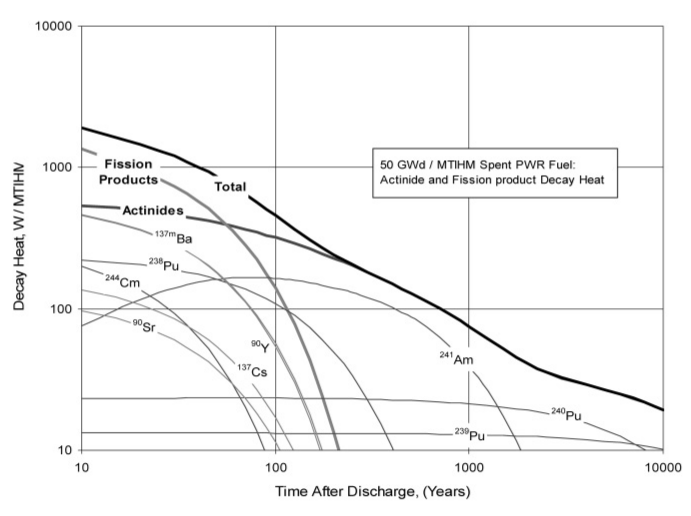
\includegraphics[scale=0.6]{./images/decay_heat.png}
	\end{center}
	\caption{Decay heat contributions in \gls{UNF} from a \gls{PWR} irradiated
		to 50 GWd/MTHM. Reproduced from Wigeland, 2006 \cite{wigeland_separations_2006}.}
	\label{fig:decay_heat}
\end{figure}


There are two major reprocessing technologies:
methods that use low-temperature chemical separation
using organic solvents (e.g. PUREX \cite{baumgaertner_purex_1976}), and
methods that use high-temperature molten salts and metals, like pyroprocessing
\cite{laidler_development_1997}. These methods separate the \gls{UNF}
into different streams, which are then sent to either a \gls{HLW} repository
(fission products) or an appropriate fuel fabrication facility (plutonium).

Different closed fuel cycles use different elemental groups for recycled
fuel fabrication. For example, the PUREX process is used in La Hague in France
\cite{schneider_spent_2008}, THORP in the U.K \cite{riley_technology_1998},
Mayak in Russia, and Rokkasho in Japan to separated plutonium and uranium
\cite{birkett_recent_2005}. The plutonium is mixed with either depleted
uranium (tails) or reprocessed uranium to produce \gls{MOX}.

Closed fuel cycles
generally involve fast-spectrum reactors to control TRU inventory.
A fast-spectrum reactor can be designed to either burn (reduce TRU),
breed (produce more TRU), or break-even (maintain TRU amount).
Selection of the fast-spectrum reactor design depends on the
goal of the deploying institution.


\subsubsection{Fuel cycle with limited recycling}
Fuel cycle with limited recycling is when the \gls{UNF}
is recycled for a limited number of times. 
The purposes for recycling the irradiated fuel include
reusing the separated material in a nuclear reactor, or 
separating long-lived highly radioactive elements
for repository burden reduction \cite{wigeland_nuclear_2014}.
The difference
between limited recycling and `closed' fuel cycles (continuous
recycling) is that continuous recycling always reprocesses
irradiated fuel and only disposes \gls{HLW}, while limited
recycling fuel cycles dispose some irradiated fuel.


\subsection{Fuel Cycle Transition Scenarios}
Fuel cycle transition scenarios are when an initial
fleet of technologies and corresponding fuel cycle strategies
dynamically evolve into a different final state \cite{oecd_nuclear_2009}.
In this work, I focus on the transition from
once-through fuel cycles to closed fuel
cycles through the progressive replacement of previous technology
(i.e. \glspl{LWR}) with an advanced technology (i.e. reprocessing
and fast-spectrum reactors). Other transition scenarios include
a general transition into a different fuel cycle (evaluation group
defined by Wigeland et al.) or to a mixture of fuel cycles, or
a complete nuclear energy phaseout.

Analysis of transition scenarios requires
deliberate tracking of materials and facilities in order
to accurately calculate the resources necessary for a
successful transition.

The timescale and feasibility of a transition scenario
varies by nation, depending on the nation's nuclear energy demand,
fuel cycle strategies, and initial conditions.
In this work, I only consider the material feasibility of the
transition scenario. Economic and political feasibility analyses
are out of the scope of this work. A fuel cycle transition is considered
materially feasible if all the deployed reactors receive fuel
in time.

The fuel demand is determined by two factors - nuclear energy demand
and the nation's fuel cycle strategy.
The nuclear energy demand determines the construction
and operation
schedule of new reactors, and the fuel demand is
calculated accordingly.
Fuel cycle strategies determine the isotopic
requirement of the fuel cycle transition scenario. For example,
if the transition drives toward a U-Pu \gls{MOX} fuel cycle,
plutonium inventory dominates the timescale and feasibility of transition.

Once the expected fuel demand is calculated,
the initial condition - current fissile material inventory
and reactors (and their remaining lifetimes) - determines
the material feasibility and timescale of a transition scenario.
If a transition scenario is infeasible (i.e. fissile source is lacking),
the transition can be `loosened', by delaying deployment
of advanced reactors. The energy demand is instead met by additional
deployment of previous reactor technology (e.g. \glspl{LWR}),
thereby increasing transition timescale but reducing the
intensity of fissile material demand.

Determining material feasibility of a \gls{NFC} transition scenario
requires dynamic tracking of material flows from multiple facilities,
as well as modeling of complex systems. This work
determines material feasibility by calculating
the material inventory of real-world \gls{NFC} transition scenarios.


\section{Objectives}

This thesis demonstrates and extends the real-world \gls{NFC} transition
scenario modeling capabilities in Cyclus. 
The goal is to
develop tools that leverage Cyclus' modularity to
add capabilities required for modeling real-world
fuel cycle transition scenarios, and demonstrate Cyclus'
capabilities by using the developed tools to perform
\gls{NFC} transition scenarios relevant to France and the United
States.

\section{Methods}
This thesis accomplishes the objective in three steps. 
First, a benchmark showed good agreement with other
fuel cycle simulation tools. \footnote{These results have been
submitted for publication in Annals of Nuclear Energy.}
Second, I identified and developed the tools and methods necessary
for modeling and simulating real-world transition scenarios.
Finally, I constructed and ran fuel cycle transition scenarios
relevant to France and the United States.

\subsection{Benchmark study}
A previous study by Feng et al. \cite{feng_standardized_2016} validates existing 
\glspl{NFCS} in a fuel cycle transition scenario, in which an \gls{LWR} fleet
transitions into an \gls{SFR} fleet with continuous reprocessing. This 
study compares four well-known \glspl{NFCS}
DYMOND \cite{yacout_modeling_2005},
VISION \cite{jacobson_verifiable_2010},
ORION \cite{gregg_analysis_2012}, and
MARKAL \cite{shay_epa_2006}. The results from each code were
compared to a set of `model solutions' that were generated
from a spreadsheet for various metrics (e.g. fuel loading
in reactor, \gls{UNF} inventory). I reproduced the transition
scenario in Cyclus, and compare the Cyclus results with those
from the model solutions.

\subsection{Tool development}
In order to model real-world transition into an advanced
fuel cycle, I developed two major tools. First, I developed \texttt{write\_input.py}
that automates extraction from the curated \gls{IAEA} \gls{PRIS} database
\cite{iaea_nuclear_2018}. The database lists each nuclear reactor's
country, name, type, net capacity (\gls{MWe}), status, operator, construction
date, first criticality date, first grid date, commercial date, and shutdown
date (if applicable). \texttt{write\_input.py} extracts the information from this file
to generate a Cyclus compatible input file, which lists the individual
reactor units as agents. Second, I developed a module that models \glspl{MSR}
in Cyclus using a database generated from a high-fidelity \gls{MSR} depletion calculation.
The database is an output of SaltProc \cite{rykhlevskii_arfc/saltproc:_2018}, a python
module that drives
SERPENT 2 \cite{leppanen_serpentcontinuous-energy_2013} to model online reprocessing in an \gls{MSR}.
The database contains the historic compositions of each stream in and out of the reactor,
composition history inside the reactor, and $k_{eff}$ values. The developed tool then
reads the database to mimic \gls{MSR} behavior by requesting and offering
feed and waste material to the Cyclus framework. The database is in HDF5
format, a hierarchical data format designed to store and organize
large amounts of data \cite{the_hdf_group_hierarchical_1997}.

Finally I constructed the fuel cycle transition scenario for France and the United States.
I made different assumptions for the two scenarios to account for each nation's different goals,
initial conditions (i.e. currently existing fleet, \gls{UNF} inventory), and their potential reactor
technology. I used the \texttt{write\_input.py} to construct the initial Cyclus input file,
followed by iterations to account for new reactor deployment. The workflow driving the analyses is shown in diagram \ref{diag:workflow}.


\begin{figure}
        \centering
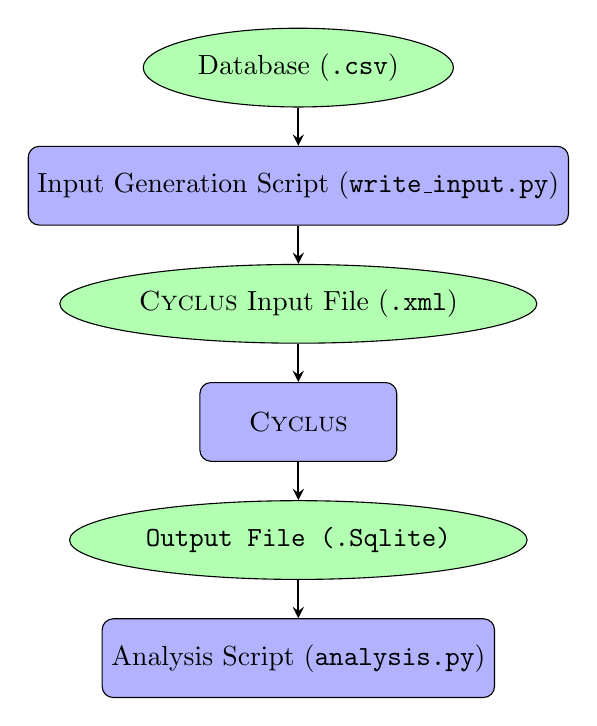
\begin{tikzpicture}[node distance=1.5cm]
\node (database) [object] {Database (\texttt{.csv})};
\node (script) [process, below of=database] {Input Generation Script (\texttt{write\_input.py})};
\node (input) [object, below of=script] {\Cyclus Input File (\texttt{.xml})};
\node (cyclus) [process, below of=input]{\Cyclus};
\node (output) [object, below of=cyclus]{\texttt{Output File (\texttt{.Sqlite})}};
\node (script2) [process, below of=output]{Analysis Script (\texttt{analysis.py})};

\draw [arrow] (database) -- (script); 
\draw [arrow] (script) -- (input); 
\draw [arrow] (input) -- (cyclus);
\draw [arrow] (cyclus) -- (output);
\draw [arrow] (output) -- (script2);
\end{tikzpicture}
\caption{Green circles and blue boxes represent files and software 
processes, respectively, in the computational workflow.}
\label{diag:workflow}
\end{figure}


The structure of this thesis is as follows. In chapter 2, I review other fuel cycle simulation
tools and their gaps, and explain the unique capability Cyclus
has for transition scenario simulation.
Chapter 3 shows the design and
development of capabilities needed for \gls{NFC} transition simulation.
Chapter 4 shows the results from the benchmark study, in which Cyclus results are compared
to results from other fuel cycle simulation tools.
Chapter 5 and 6 show the results from the France and United States fuel cycle
transition scenario.


\chapter{Nuclear Fuel Cycle Simulators}
\glspl{NFCS} are system-level analysis tools
that allow tracking of material flow in a \gls{NFC}. Its
functionalities include, but are not limited to, isotopic decay,
depletion calculations, and separating of material streams.
The goal of a \gls{NFCS} is to calculate `metrics' - quantitative
measures of performance that can be compared among fuel cycle
options \cite{huff_fundamental_2016}.

\section{Capabilities required for modeling transition scenarios}
There are specific capabilities required for modeling transition
scenarios. A study by Brown et al. \cite{brown_identification_2016}
identified nine common functionalities for \glspl{NFCS} for modeling
transition scenarios - material compositions, deployment of fuel
cycle facilities, front-end facility models, separations and material
recycle facilities, reactor facilities, back-end features, starting
the new fuel cycle, materials queuing and prioritization under
capacity limitations, and energy demand algorithms. Brown et al.
categorizes each functionality into three tiers - basic, integral,
and exemplary. The functionalities, features, and their hierarchies
are organized in table \ref{tab:ffh}.

\begin{table}[h]
    \centering
    \caption {Nine common functionalities identified for \gls{NFCS} to perform
    			fuel cycle transition scenarios. Reproduced from Brown et al. \cite{brown_identification_2016}}
    \label{tab:ffh}
    \begin{tabular}{lll}
        \hline
        \textbf{Functionality}&\textbf{Feature} &\textbf{Hierarchy} \\
        \hline
        \multirow{6}{*}{\shortstack{Composition \\ Features}} & \shortstack{Modeling of implicit consideration of fuel materials \\  including primary fissile and fertile actinide isotopes} & Basic \\
        	& \shortstack{Fuel's initial heavy metal mass modeled as lumped masses \\ of the remaining actinides and fission products to conserve mass} & Basic \\
        	& Isotopic decay of materials in storage & Exemplary \\
        	& Modeling of intermediate isotopes (e.g. Pa-233) & Exemplary \\
        	& Tracking of fission products beyond a simple lumped sum & Exemplary \\
        	& Modeling of compounding materials in fuels and waste forms & Exemplary\\

        \hline

        \multirow{3}{*}{\shortstack{Fuel Cycle \\ Facility \\ Deployment}} & Facility deployment and retirement & Basic \\
        	& Construction time delays & Basic \\
        	& Strategic deployment to meet demand &Integral \\

        \hline

        \multirow{6}{*}{\shortstack{Front-end \\ Facilities}} & Source (mining and milling) & Basic \\
        	& Details of mines and mills including annual and total quantities available & Exemplary \\
        	& Conversion and enrichment facilities & Basic \\
        	& Timing and capacity of recycle facilities & Basic \\
        	& Fuel fabrication & Basic \\
        	& Time delays and losses in separations and fabrication & Basic \\

        \hline

        \multirow{4}{*}{\shortstack{Separations \\ and \\ Material \\ Recycling}} & Separations facilities may be required for \gls{UNF} & Basic \\
        	& Cooling time & Basic \\
        	& Losses in separations & Basic \\
        	& Material selection from the \gls{UNF} supply & Basic \\

        \hline

        \multirow{6}{*}{\shortstack{Reactor \\ Facility}} & Fueling: number of batches, cycle length and fuel per batch & Basic \\
        	& Multiple fuel types in reactor facility (driver, blanket) & Basic \\
        	& Pre-generated charge and discharge isotopic compositions & Basic \\
        	& Real time calculations based on reactor physics models & Exemplary \\
        	& Reactor facility lifetime, construction time, and decommissioning time & Basic \\
        	& Initial charge for first core and discharge for final core & Basic \\

        \hline

        \multirow{2}{*}{Back-end} & Cooling of used fuel & Basic \\
        	& \shortstack{Conservation of mass - consistency with\\ charged mass and generated power} & Basic \\

        \hline

        \multirow{3}{*}{\shortstack{Fuel Cycle \\ Startup}} & External source of fissile material & Basic \\
        	& Startup on recycled fuel from other facilities &Integral \\
        	& Primary and back-up fuel types & Exemplary \\

        \hline

        \multirow{3}{*}{\shortstack{Material \\ Prioritization}} & material accumulation & Basic \\
        	& Material prioritization &Integral \\
        	& Radioactive decay & Exemplary \\

        \hline

        \multirow{2}{*}{\shortstack{Energy Demand \\ Algorithm}} & Technology allocation accounting for availability &Integral \\
        	& Ordering and deployment of multiple reactor technologies &Integral \\
        \hline
    \end{tabular}
\end{table}

\section{Additional capabilities identified for real-world fuel cycle transition scenario}
From the functionalities identified in Brown et al., I identified two additional functionalities -
modeling discrete, real-world reactor fleets and operational history; modeling liquid-fueled
reactors with continuous reprocessing.

\subsection{Modeling discrete, real-world reactor fleets}
For modeling real-world nuclear fuel cycle transition scenarios, the initial
condition (e.g. existing fissile inventory, existing reactor fleet) is important
to understand transition parameters, such as transition rapidity.

\glspl{NFCS} like COSI 6 \cite{meyer_new_2009}, EVOLCODE \cite{alvaerz-velarde_validation_2014},
FAMILY21,
do have discrete facility modeling capabilities, while ORION \cite{},
DESAE2.2\cite{tsibulskiy_desae_2006}, and VISION \cite{jacobson_verifiable_2010} does not \cite{boucher_international_2010}.
However,

Only one published study is done modeling the current U.S. nuclear fleet,
using ORION \cite{sunny_transition_2015}. This is done using 





\subsection{Modeling liquid-fueled reactors with continuous reprocessing}
\glspl{MSR} reactor designs have recently gained attention due to it being a
potentially safer, more efficient, and sustainable form of nuclear power
\cite{serp_molten_2014}. Multiple companies in the U.S. are now pursuing
commercialization of \gls{MSR} design reactors, such as Tranasatomic \cite{transatomic_technical_2016}
, Terrapower, Terrestrial \cite{leblanc_18-_2017}, and
Thorcon \cite{dolan_19-_2017}. Other parties such as China (TMSR-LF \cite{dai_17-_2017}) 
and the European Union (MSFR \cite{heuer_towards_2014}, MOSART \cite{ignatiev_molten_2014})
are developing \gls{MSR} designs.

However, modeling \glspl{MSR} is difficult due to its online reprocessing regime.
The material flow in and out of the reactor is continuous and dynamic, as well as the
composition inside the core.
The neutronics and depletion calculations have to be performed continuously while
the composition of the fuel changes. Reactor physics and depletion calculations
on the \gls{MSR} have been done, notably by 
 Oak Ridge National Laboratory researchers who developed
ChemTriton \cite{powers_new_2013}, a python script that drives SCALE,
to perform semi-continuous reprocessing of the fuel \cite{powers_inventory_2014, betzler_fuel_2018}.
However, there is no existing \gls{NFCS} that has the capability to model \glspl{MSR}
due to the large computational burden associated with frequent depletion calculations.

[that's where I come in]





\section{Cyclus}




\begin{itemize}
	\item Required capabilities for modeling transition scenarios
	\begin{itemize}
		\item Real-World modeling
		\item Advanced Reactor modeling
		\item Reprocessing and transmutation
	\end{itemize}
	\item Current state of other \gls{NFCS}
	\item Current State of Cyclus
	\item Gaps in Cyclus that needs to be filled
	\item Tools developed in this paper
\end{itemize}


\chapter{Tools Used for this work}
\section{Cyclus}

\Cyclus is an agent-based fuel cycle simulation framework 
\cite{huff_fundamental_2016}, meaning
that each reactor, reprocessing plant, and fuel fabrication plant is modeled as an agent.
A \Cyclus simulation contains prototypes, which are fuel cycle facility models (archetypes) with
pre-defined parameters, that are deployed in the simulation as \texttt{facility} agents.
Encapsulating the \texttt{facility} agents are the \texttt{Institution} and \texttt{Region}.
A \texttt{Region} agent holds a set of \texttt{Institution}s. 
An \texttt{Institution} agent can deploy or decommission \texttt{facility} agents.
The \texttt{Institution} agent is part of a \texttt{Region} agent,
which can contain multiple \texttt{Institution} agents. Several versions of \texttt{Institution}
and \texttt{Region} exist, varying in complexity and functions \cite{huff_extensions_2014}.
\texttt{DeployInst} is used as the institution archetype for this work, where the institution
deploys agents at user-defined timesteps. 

At each timestep,
agents make requests for materials or bid to supply them and exchange
with one another. A market-like mechanism called the dynamic resource exchange
\cite{gidden_agent-based_2015} governs the exchanges.
For output analysis, each material resource has a quantity, composition, name, and a unique identifier.

In this work, each nation is represented as a distinct \texttt{Region} agent,
that contains \texttt{Institution} agents, each deploying  \texttt{Facility} 
agents. The \texttt{Institution} agents then deploy agents according to 
a user-defined deployment scheme.

The Cyclus \gls{NFCS} framework and its
modeling ecosystem, the suite of agents and other
physics plug-in libraries compatible with it, incorporate
modern insights from simulation science and software
architecture \cite{huff_fundamental_2016}. Cyclus
has a multitude of benefits from other available
\glspl{NFCS} codes - open-sourceness, modularity,
and extensibility. Its agent-based modeling approach
is ideal for modeling coupled, physics dependent
supply chain problems common in \glspl{NFC}.
The framework allows for dynamic loading of 
external libraries, which allows the users to plug-and-play
different types of physics models for \gls{NFC}
simulation.

\subsection{Open Source}
License agreements and institutional
approval is need for most \glspl{NFCS} like COSI, DANESS, DESAE, EVOLCODE,
FAMILY21, NFCSim, ORION and VISION \cite{juchau_modeling_2017}, making
it hard for both the usage and development in an academic settings.
On the other hand, Cyclus relies completely on open source,
free libraries, allowing all users to both use and develop the
Cylcus framework and existing libraries. The open-sourceness
of Cyclus encourages collaboration - any user can propose
improvements or provide input for Cyclus.

\subsection{Modularity and Extensibility}
In most modern \glspl{NFCS}, the facilities and their
behavior (and its fidelity) is confined in the software.
Also, most modern \glspl{NFCS} are restricted to model
a set of fuel cycles (once-through, continuous reprocessing)
with restrictions to connections between facilities. On the
other hand, Cyclus allows users to plug-and-play different libraries
that contain different fidelity modules within the Cyclus framework
(shown in figure \ref{fig:core}).
Also, the Cyclus simulation relies on a market-based model
for material trades between facilities, so the user can design
any novel fuel cycle. Also, this gives Cyclus the option to not
be limited to nuclear fuel cycles, but any system analysis
involving multiple connected facilities with physics-based
calculations.


\begin{figure}[htbp!]
	\begin{center}
		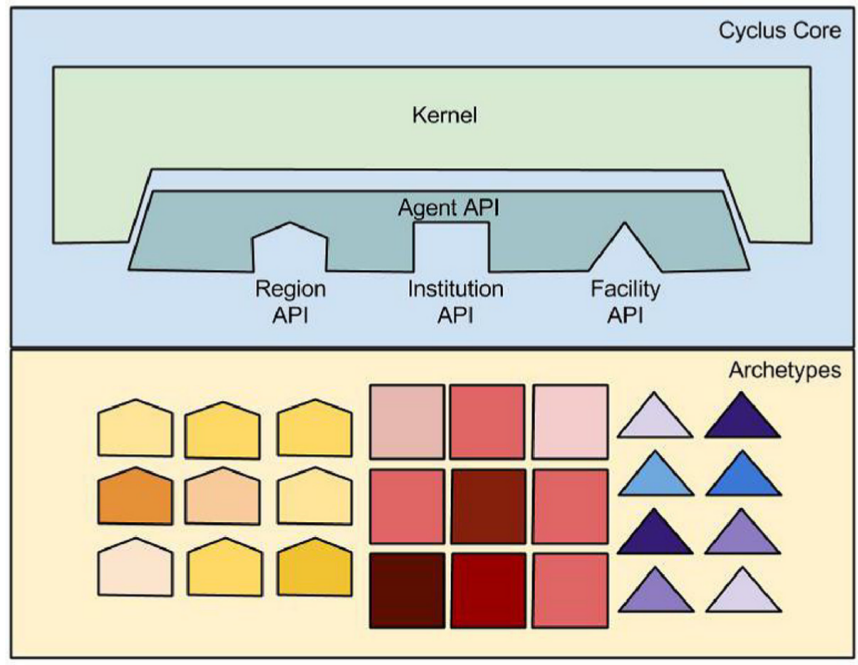
\includegraphics[scale=0.2]{./images/cyclus_core.png}
	\end{center}
	\caption{The Cyclus core provides APIs that allows the archetypes
			to be loaded into the simulation in a module fashion
			\cite{huff_fundamental_2016}.}
	\label{fig:core}
\end{figure}

The connection between the framework and the agents is
the dynamic resource exchange (DRE), where the agents
interact with each other through material offers and requests.
The kernel solves the material offers and requests, and executes
the transaction between two agents.

\subsection{Cyclus' fitness for real-world \gls{NFC} transition scenario}
The Cyclus framework and its extension libraries fulfill all the functionalities
specified by Brown et al. \cite{brown_identification_2016}.  Additionally,
its text-based input structure and discrete facility modeling capabilities
allow modeling of real-world, individual reactors. Finally, 
the addition of a \gls{MSR} model can be achieved without altering
Cyclus due to its modularity. The details of the implementation
of these capabilities are shown in the next chapter.



\section{SaltProc}
\label{sec:saltproc}

SaltProc is an on-line reprocessing simulation
driver for SERPENT2 \cite{leppanen_serpent_2015} by Andrei Rykhlevskii,
for simulating liquid-fueled \gls{MSR} operation \cite{rykhlevskii_arfc/saltproc:_2018}.
SaltProc uses a semi-continuous approach to simulate
continuous \gls{MSR} material feed and removal \cite{rykhlevskii_online_2017}.
It is coded in Python (compatible with both Python 2 and 3), and
records feed, removal, and in-core isotopic history in an HDF5 \cite{the_hdf_group_hierarchical_1997} database.

SaltProc's structure and capabilities are similar to that of the
ChemTriton tool for SCALE, developed at ORNL \cite{betzler_molten_2017}.
The computationally heavy work - Monte Carlo neutron transport and
burnup calculations - is done in SERPENT, while SaltProc parses through
the output material compositions, processes the fuel (removal and feed),
and creates a new SERPENT input file. The user can specify removal
rates, feed rates, and removal efficiencies for each isotope. At each
timestep, the following stream composition vectors are recorded in the database:
\begin{itemize}
	\item depleted core
	\item depleted core after reprocessing
	\item removal stream (reprocessed elements)
	\item feed stream
\end{itemize}


The logical flow of SaltProc is illustrated in figure \ref{fig:SaltProc}.
Initially, SaltProc reads a user-defined SERPENT 2 input file that
contains parameters such as  geometry, non-fuel component composition,
neutron population, criticality cycles, depletion time, total power, and boundary conditions.
SERPENT 2 then performs neutron transport and depletion calculations and 
returns the number density of the depleted fuel. SaltProc then reads the
depleted composition, writes the composition in the database, processes
the depleted material according to a user-defined scheme, and then
outputs a new fuel composition input card for SERPENT 2. This again
is then read by SERPENT 2 and the cycle continues until the user-defined
timestep is reached.

\begin{figure}[htbp!]
	\begin{center}
		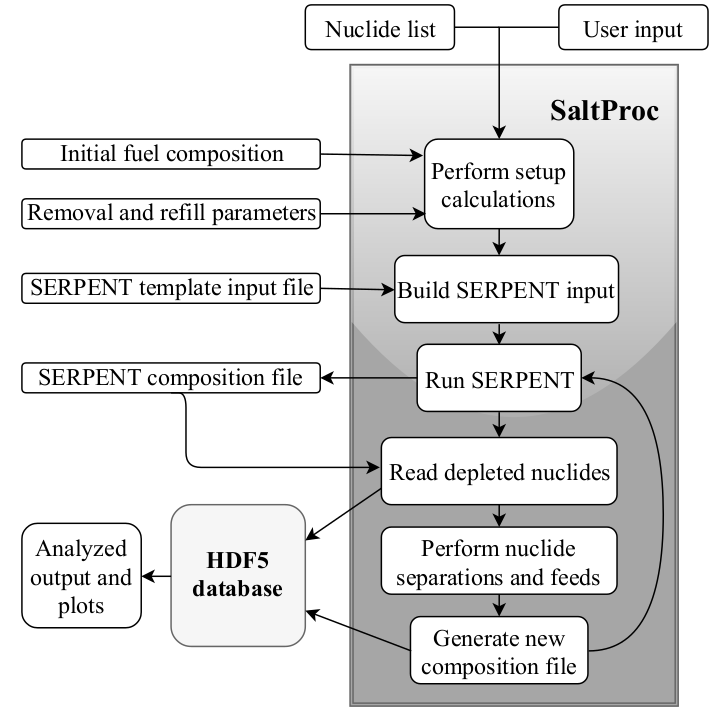
\includegraphics[scale=0.5]{./images/saltproc.png}
	\end{center}
	\caption{Flow chart for the SaltProc tool
		\cite{rykhlevskii_online_2017}.}
	\label{fig:SaltProc}
\end{figure}


One of the benefits of having a semi-continuous external driver for
SERPENT 2 is that the user can set up SaltProc so that the density
of a certain isotope in the fuel remains constant. In other words,
the feed rate can vary over time to meet a certain `quality' of the fuel.
Also, using a Monte Carlo code such as SEPRENT allows users to vary
geometric fidelity, from a single cell model to a full core model.

\subsection{Use in this work}
SaltProc's output (in HDF5 \cite{the_hdf_group_hierarchical_1997} format) can be imported through a \Cyclus
module to mimic the \gls{MSR} feed and removal
behavior throughout its lifetime. The composition in the core is
not important here since the data of interest in a system-level \gls{NFC} simulation
is the material flow in and out of the reactor. This method can
effectively model \glspl{MSR} in a large system-scale \gls{NFC}
simulation without significant computational burden for the \gls{NFC} simulation at run-time.

\chapter{Tools developed for this work}
I developed two extensions to leverage 
the capabilities of \Cyclus to model
real-world fuel cycle transition scenarios.
The first extension is a python input-generating module
that automates scenario generation of the real-world 
nuclear fleet at any point in time. The second extension
is a \Cyclus archetype that mimics \gls{MSR} feed and removal
behavior using an HDF5 database generated from SaltProc.

\section{\texttt{cyclus-input-gen}}
\label{sec:writeinput}
The python package \texttt{cyclus-input-gen} contains
multiple submodules for automating \Cyclus input generation.
The submodule \texttt{from\_pris} automates the generation of \Cyclus input files
to model the state of reactor fleets at a given
point in time.

The script reads from the \glsfirst{PRIS} database \cite{iaea_nuclear_2018}
and extracts data about each reactor's country, reactor unit,
type, net capacity (MWe), status, operator, construction date,
first criticality date, first grid date, commercial date,
and shutdown date (if applicable). The user inputs simulation
configurations such as start year, start month, and
simulation duration. \texttt{from\_pris} uses the collected data to
fill out a template into a \Cyclus input file. 
Diagram \ref{diag:log_flow} shows the logical flow of the module.


\begin{figure}
	\centering
	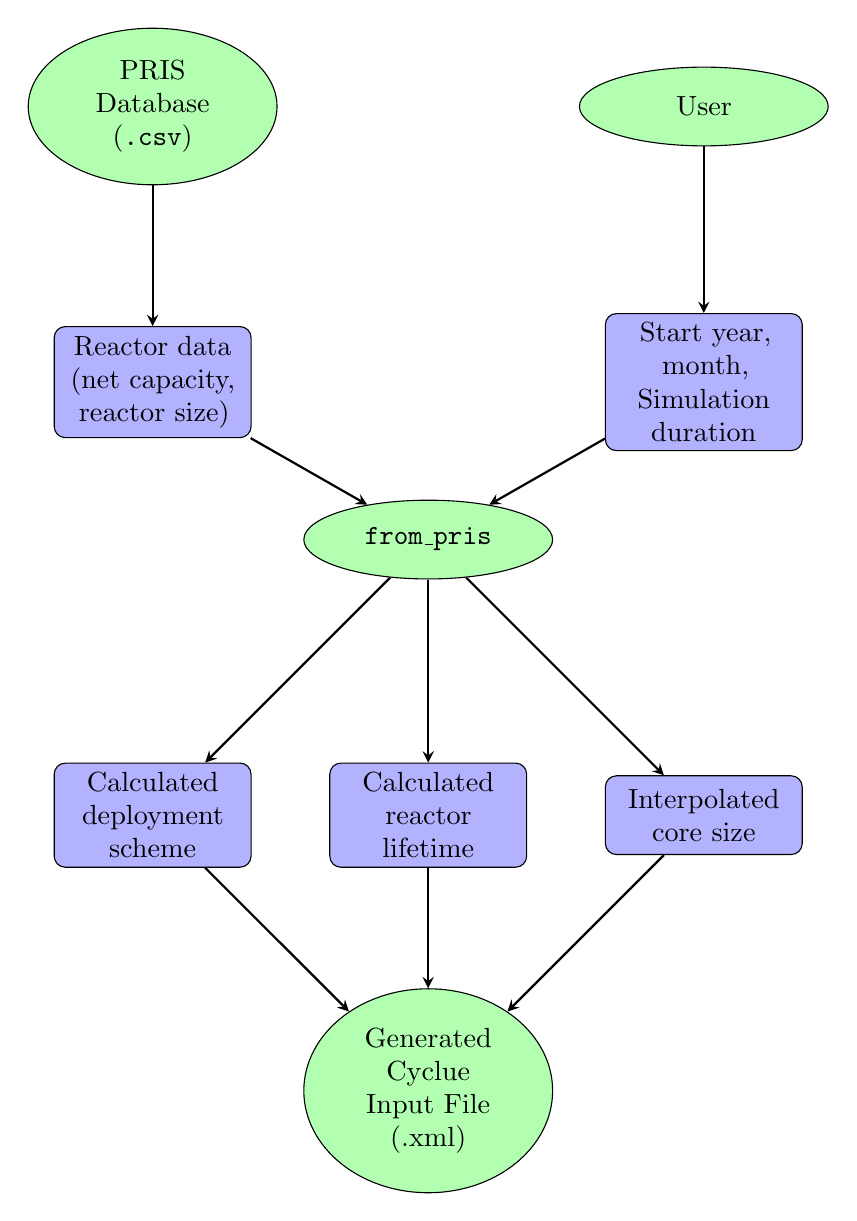
\begin{tikzpicture}[node distance=3.5cm and 2cm, on grid, auto, text width=2cm]
	\node (database) [object] {PRIS Database (\texttt{.csv})};
	\node (data) [process, below of=database] {Reactor data (net capacity, reactor size)};
	
	\node (user) [object, right=7cm of database] {User};
	\node (input) [process, below of=user] {Start year, month,  Simulation duration};
	
	\node (script) [object, below right= 2cm and 3.5cm of data] {\texttt{from\_pris}};
	
	\node (lifetime) [process, below of=script] {Calculated reactor lifetime};
	\node (coresize) [process, right of=lifetime] {Interpolated core size};
	\node (region) [process, left of=lifetime] {Calculated deployment scheme};
	
	\node (output) [object, below of=lifetime] {Generated Cyclue Input File (.xml)};
	
	\draw [arrow] (database) -- (data); 
	\draw [arrow] (user) -- (input); 
	\draw [arrow] (data) -- (script);
	\draw [arrow] (input) -- (script);
	
	\draw [arrow] (script) -- (lifetime);
	\draw [arrow] (script) -- (coresize);
	\draw [arrow] (script) -- (region);
	
	\draw [arrow] (lifetime) -- (output);
	\draw [arrow] (coresize) -- (output);
	\draw [arrow] (region) -- (output);
	
	\end{tikzpicture}
	\caption{ Logic flow of \texttt{from\_pris}.
		Green circles and blue boxes represent files and data, respectively.}
	\label{diag:log_flow}
\end{figure}

\subsection{Reactor deployment calculation}
The module calculates the deployment
scheme of reactors and their lifetimes by assuming
that all reactors shut down after 60 years of operation.
If the expected shutdown date is later than the user-input
simulation start date,
the reactor is not written in the input. If the reactor was
operational prior to the simulation start date,
and its shutdown date later than simulation start date,
the reactor is deployed at the beginning of simulation with its remaining lifetime.
If the reactor's start date is later than the simulation
start date, and the shutdown time is undefined, the reactor
is deployed at the defined start date with 60 years of lifetime.

\subsection{Reactor parameter calculation}

The module calculates the core sizes of various reactor
types by using a linear core size model. It assumes that
the number of assemblies in a 
reactor core scales linearly from a model reactor design,
as shown in the equation below. The mass per assembly
is kept constant.
The model reactor designs are listed in table \ref{tab:lin_core}.

\[
A = A_{ref} \cdot \frac{\text{P}}{P_{ref}}
\]
\[
N_{assem.pwr} = 157 \cdot \frac{\text{P}}{1,100}
\]
\[
N_{assem.bwr} = 764 \cdot \frac{\text{P}}{10,098}
\]
\[
N_{assem.phwr} = 4,560 \cdot \frac{\text{P}}{700}
\]
\[
A = \text{number of assemblies in approximated core}
\]
\[
P = \text{power capacity of reactor}
\]

\begin{table}[h]
	\centering
	\caption{Reactor model designs used for the linear core size model.}
	\begin{tabularx}{\textwidth}{zzqqq|q}
		\hline
		\textbf{Category} & \textbf{Model Reactor} & \textbf{Power [MWe] ($P_{ref}$)} & \textbf{Assembly Mass [kg]} & \textbf{Assemblies in Core ($A$)} & \textbf{Reference}  \\
		\hline
		\gls{PWR} & AP-1000 & 1,110 & 446 & 157 & \cite{schulz_westinghouse_2006} \\
		\gls{BWR} & 4-MK I & 1,098 &180 & 764 & \cite{moore_physical_1989} \\
		\gls{PHWR} & CANDU6 & 700 & 24.17 & 4,560 & \cite{galeriu_technical_nodate} \\
		\hline
	\end{tabularx}
	\label{tab:lin_core}
\end {table}



\section{saltproc\_reactor}
The SaltProc reactor is a \Cyclus facility archetype designed to 
model \gls{MSR} behavior using a database. It roughly couples ``SaltProc'' \cite{rykhlevskii_online_2017}
and \Cyclus, by using the output from SaltProc to mimic \gls{MSR}
feed and removal behavior in \Cyclus.

This method is similar to the simplified implementation of
recipe reactors, in which the depletion calculation is performed outside of the
fuel cycle simulation. Instead of a single depletion calculation
used in a recipe reactor, this reactor uses a database of recipes
to capture the continuously varying state of liquid-fueled reactors like \glspl{MSR}. 


\begin{figure}
	\centering
	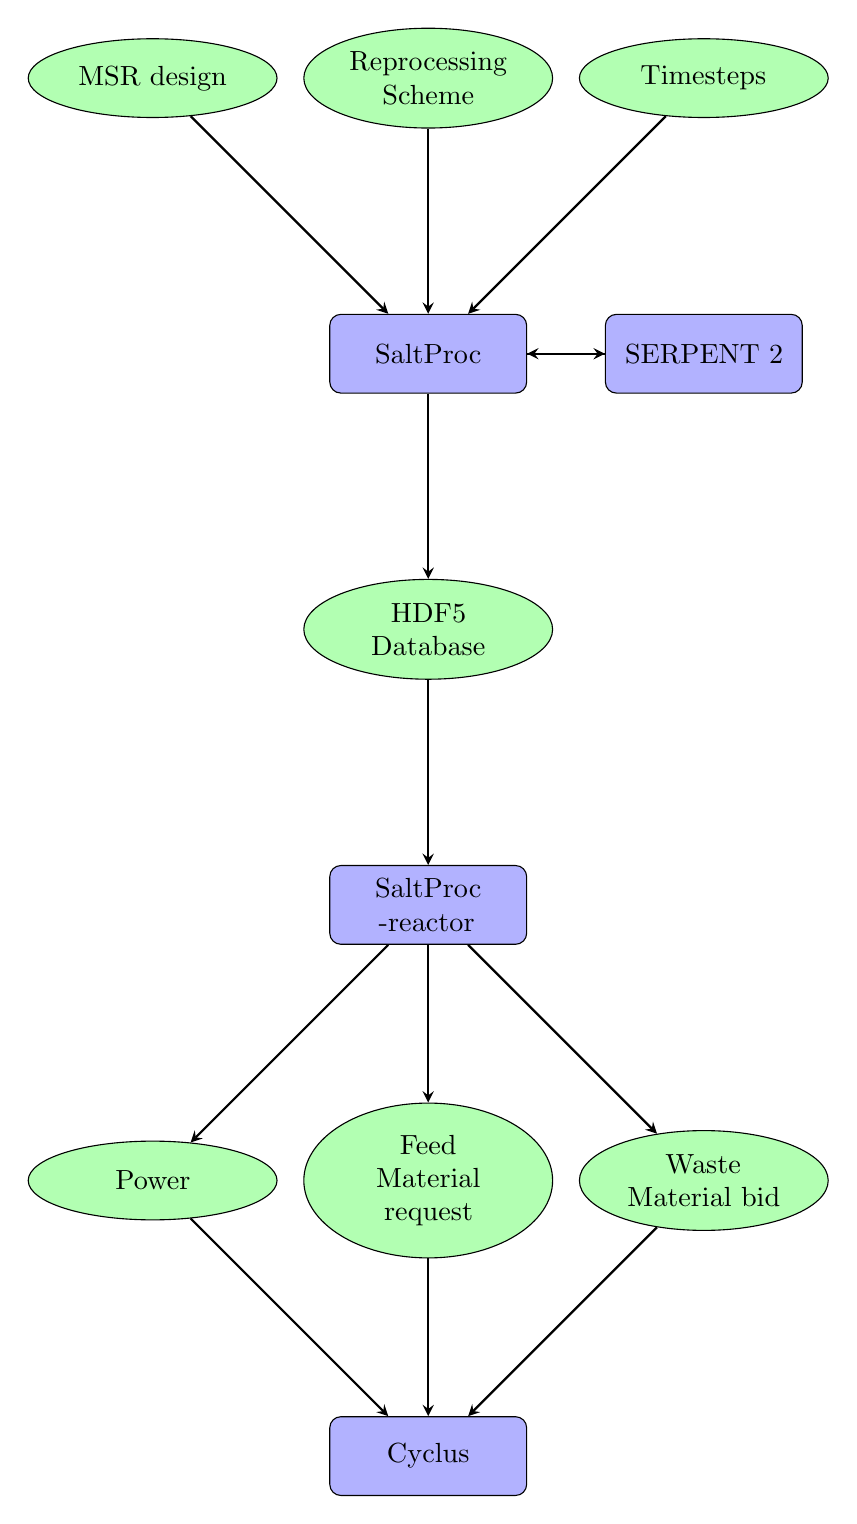
\begin{tikzpicture}[node distance=3.5cm and 2cm, on grid, auto, text width=2cm]
	
	\node (msr) [object] {\gls{MSR} design};
	\node (repro) [object, right of = msr] {Reprocessing Scheme};
	\node (timesteps) [object, right of = repro] {Timesteps};
	
	\node (saltproc) [process, below of = repro] {SaltProc};
	\node (serpent) [process, right of = saltproc] {SERPENT 2};
	
	\node (hdf5) [object, below of = saltproc] {HDF5 Database};
	
	\node (hdf5 reactor) [process, below of = hdf5] {SaltProc -reactor};
	
	\node (bid) [object, below of = hdf5 reactor] {Feed Material request};
	\node (request) [object, right of = bid] {Waste Material bid};
	\node (power) [object, left of = bid] {Power};
	
	\node (cyclus) [process, below of = bid] {Cyclus};


	\draw [arrow] (msr) -- (saltproc); 
	\draw [arrow] (repro) -- (saltproc); 
	\draw [arrow] (timesteps) -- (saltproc);
	
	\draw [arrow] (saltproc) -- (serpent);
	\draw [arrow] (serpent) -- (saltproc);
		
	\draw [arrow] (saltproc) -- (hdf5);
	\draw [arrow] (hdf5) -- (hdf5 reactor);
	
	\draw [arrow] (hdf5 reactor) -- (bid);
	\draw [arrow] (hdf5 reactor) -- (request);
	\draw [arrow] (hdf5 reactor) -- (power);
	
	\draw [arrow] (bid) -- (cyclus);
	\draw [arrow] (request) -- (cyclus);
	\draw [arrow] (power) -- (cyclus);
	
	
	\end{tikzpicture}
	\caption{ Logic flow of \texttt{SaltProc Reactor}.
		Green circles and blue boxes represent files and data, respectively.}
	\label{diag:hdf5_flow}
\end{figure}

\subsection{Code description}
The user provides only of the commodity names
for each stream (e.g. waste, fertile), and the database path, since the
HDF5 database already contains the notion of reactor design,
reprocessing scheme, and other reactor parameters (shown in
figure \ref{diag:hdf5_flow}). The commodity names are needed
for reactor agents to communicate with other \Cyclus agents
in exchanging material.

At every timestep, 
The \texttt{SaltProc Reactor} calculates the material mass
and composition accumulated during the \Cyclus timestep,
as shown in equation below.

\[
M_{T} = \sum m_T
\]
\[
m_{T} = \sum_{t=(T-1)}^{T} m_{t}
\]
\[
M_T = \text{total mass of stream in one \Cyclus timestep}
\]
\[
m_T = \text{mass of isotope in one \Cyclus timestep}
\]
\[
m_t = \text{mass of isotope in one SaltProc timestep}
\]


\section{Limitations of the database approach}
\label{sec:limit}
The limitations of this database approach are that it does not
take into account the changing incoming fuel compositions due to decay.
The separated \gls{TRU} composition may vary depending on the time
an \gls{LWR} \gls{UNF} assembly has been cooled, thus affecting the performance
of the \gls{MSR}. The database approach assumes a fixed input salt
composition, which is not the case in this simulation, because reprocessed
\gls{TRU} has varying decay times from discharge when it is fabricated and
put in the \gls{MSR}.

This limitation is similar to that of batch-wise recipe reactors, in which the 
pre-generated recipe already results in a depleted fuel composition that is agnostic to the incoming
fuel composition in the simulation. For example, a batch-wise recipe reactor
depleting a \gls{MOX} fuel would deplete the \gls{MOX} fuel to the same
composition regardless of its fresh plutonium content. This is mediated by using
a fuel fabrication facility that modifies the plutonium enrichment to
meet a certain fissile value (in \Cyclus, the Cycamore \texttt{FuelFab} archetype).

The same method can be applied such that, instead of using a fixed mass ratio
to fabricate fuel for \glspl{MSR}, the fuel fabrication is done by modifying
the \gls{TRU} enrichment to match a certain fissile value. 

Another way to overcome this limitation is to use a set of databases 
that contain multiple SaltProc simulation results with varying initial \gls{TRU}
vectors. When the reactor archetype receives the fuel, it will find the
SaltProc simulation result with the initial fuel composition closest to that
of the received fuel salt, minimizing error stemming from varying
\gls{TRU} compositions.

The best solution is to have a built-in depletion calculation model. However,
as mentioned before, this requires too much computational burden for a fuel cycle simulation,
in which there are multiple reactors `at play' at any given time. Another
possible method is to implement a reduced-order-model of \gls{MSR} depletion
behavior created by training from a large dataset of \gls{MSR} depletion
calculations.

\chapter{Cyclus benchmark Study}
This chapter demonstrates Cyclus' agreement with other
\glspl{NFCS} by benchmarking the results of Cyclus to
a previous verification study by Feng et al. \cite{feng_standardized_2016}.
This verification study compared four well-known \glspl{NFCS}
DYMOND \cite{yacout_modeling_2005},
VISION \cite{jacobson_verifiable_2010},
ORION \cite{gregg_analysis_2012}, and
MARKAL \cite{shay_epa_2006}. The results from each code were compared to a
set of `model solutions' that were generated from a spreadsheet
for various metrics (e.g. fuel loading in reactor, \gls{UNF} inventory)
in a transition scenario. I took the input parameters from this study,
and reproduced the transition scenario in Cyclus, and compare the results.
Results show that Cylcus' results are in good agreement with the results
from Feng et al., with minor differences caused by reactor module behavior.

\section{Methodology}

Feng et al. comprehensively defines simulation parameters
sufficient to reproduce the transition scenario in \Cyclus.
In this study, we used the \Cycamore \cite{huff_fundamental_2016}
archetype library to model
all fuel cycle facilities. \Cycamore libraries are
archetypes maintained by the core developer team.

\Cyclus results are output in either \texttt{.sqlite} or
\texttt{.h5} format. In this study, we used the
\texttt{.sqlite} format and analyzed the results
using python. The post-processed
output data was overlapped with the results with the
model solution from the verification study \cite{feng_standardized_2016}.
The input file and analysis procedures are all available on Github \cite{bae_arfc/transition-scenarios:_2018}.


\section{Fundamental Modeling Differences in \Cyclus}

\Cyclus has fundamental modeling choice differences from the fuel cycle analysis codes
used in the benchmark \cite{feng_standardized_2016}.

\Cyclus has a default time step of a month.
The verification study solutions are evaluated with 1-year time steps, so cumulative and annual averages
were used. For example, decommissioning
facilities occurs at the end of a timestep, and building facilities
occurs at the beginning of a timestep.

The \Cycamore recipe reactor depletes half of its core when decommissioned mid-cycle,
whereas the codes in the benchmark \cite{feng_standardized_2016} deplete all their reactors' fuel when decommissioned.
For this study, we changed
the \Cycamore source code to deplete all its assemblies to the depleted recipe.
Also, the \Cycamore recipe reactor treats each batch (and assembly) as a discrete
material, while some codes have continuous fuel discharge. This produces
differences in the results because the batches in the benchmark \cite{feng_standardized_2016} are in time-averaged values.
In this study, the \gls{LWR} batch size and cycle time is increased, while
decreasing the batch number to keep the core size constant. We round
up the \gls{SFR} batch number, while the batch size and cycle time are kept constant.
This increases the core size by $1.08 \%$, which is negligible, but will be
discussed in the results section.
The differences are listed in table \ref{tab:diff}.

\begin{table}[h]
	\centering
	\caption{Difference in Batch number and core size}
	\begin{tabularx}{\textwidth}{bss}
		\hline
		\textbf{Category} & \textbf{Benchmark\cite{feng_standardized_2016}} & \textbf{\Cyclus} \\
		\hline
		LWR Batches & 4.5 & 3 \\
		LWR Batch size [tHM] & 19.91 & 29.86 \\
		LWR Core size [tHM] & 89.59 & 89.59 \\
		LWR Cycle time & 1 year & 1.5 years \\
		SFR Batches & 3.96 & 4 \\
		SFR Batch size [tHM] & 3.95 & 3.95 \\
		SFR Core size [tHM] & 15.63 & 15.8 \\
		\hline
	\end{tabularx}
	\label{tab:diff}
	\end {table}

Note that the Cyclus framework code would never need to be changed.
The only change made was the \Cycamore reactor
depletion behavior at decommission due to its large impact on plutonium inventory.
The goal of this
study is to show current \Cyclus agreement with other codes and identify
differences, not to alter \Cyclus to match the other codes.

\section{Results}

We obtained the benchmark solutions through personal contact with
benchmark author Bo Feng at Argonne National Laboratory.

Figure \ref{fig:pow_plot} shows the deployed reactor capacity, and
figure \ref{fig:dep} shows the \gls{LWR} retirement and \gls{SFR}
deployment. The two plots show exact agreement with the
benchmark solutions.

\begin{figure}[htbp!]
	\begin{center}
		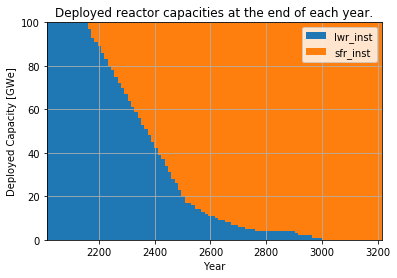
\includegraphics[scale=0.7]{./images/results_18/power_plot.png}
	\end{center}
	\caption{Deployed reactor capacities at the end of each year from Cyclus.}
	\label{fig:pow_plot}
\end{figure}


\begin{figure}[htbp!]
	\begin{center}
		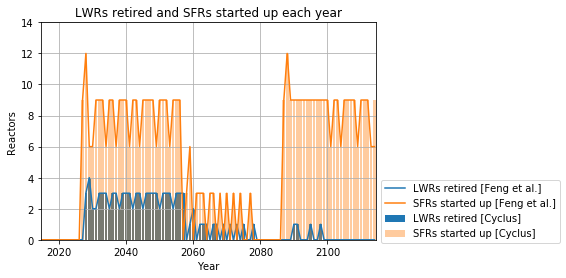
\includegraphics[scale=0.7]{./images/results_18/dep.png}
	\end{center}
	\caption{\glspl{LWR} retired and \glspl{SFR} started up each year.}
	\label{fig:dep}
\end{figure}

Figure \ref{fig:fuel_load} shows the annual fuel loading rate.
The initial fuel loading for 100 \gls{LWR} reactors are not shown in
the plot for both the benchmark and the Cyclus results.
The oscillations caused by the 18 month refueling period
were aggregated into 12 month groups. As a result the total fuel loaded
is equal for both plots.

Although indistinguishable in figure \ref{fig:fuel_load},
there is a small difference between \gls{SFR} fuel loading proportional
to the core mass difference, because Cyclus only has integer batch numbers.
Figure \ref{fig:fuel_load_diff_norm} shows the
differences normalized by the core mass differences, overlapped with the
\gls{SFR} deployment. This shows that the differences only occur during
deployment due to the difference in core mass.


\begin{figure}[htbp!]
	\begin{center}
		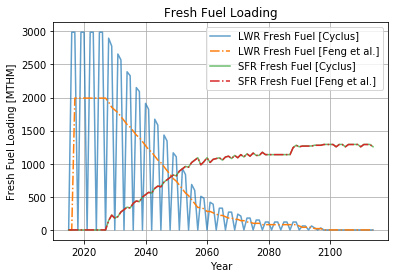
\includegraphics[scale=0.7]{./images/results_18/fuel_load.png}
	\end{center}
	\caption{Annual fresh fuel loading rates (first cores and reload fuel).}
	\label{fig:fuel_load}
\end{figure}

Figure \ref{fig:fuel_discharge_monthly} shows the inventory of discharged
\gls{UNF} in the mandatory cooling stage (four years for \gls{LWR}, one year for \gls{SFR}).
It also oscillates around the benchmark's
solution and converges, due to the influx and the outflux of \gls{UNF}
into and out of the storage facility.
The \gls{SFR} inventory and fuel loading
solutions exactly matches the benchmark solutions, minus the small ($1.07\%$) difference due to core
size.

\begin{figure}[htbp!]
	\begin{center}
		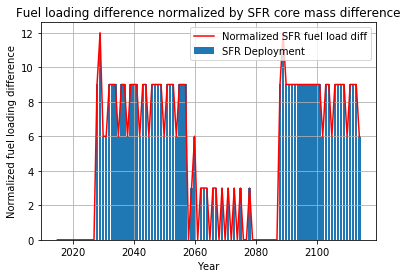
\includegraphics[scale=0.7]{./images/results_18/fuel_load_diff_norm.png}
	\end{center}
	\caption{Difference between annual fresh \gls{SFR} fuel loading rates (Cyclus - Benchmark) normalized by the core mass difference of an \gls{SFR} due to fractional batch size.}
	\label{fig:fuel_load_diff_norm}
\end{figure}


Figure \ref{fig:waiting_monthly} shows the amount of cooled \gls{UNF} waiting for
reprocessing. The value is calculated by subtracting the cumulative difference between
the cooled inventory and the \gls{UNF} reprocessing throughput.

\[ M_{wait, t} = M_{cooled, t} - M_{rep, t} \]

The oscillation is between the cooled inventory in the storage facility before (high)
and after (low) it sends its inventory for reprocessing.

\begin{figure}[htbp!]
	\begin{center}
		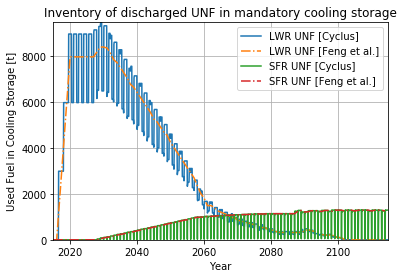
\includegraphics[scale=0.7]{./images/results_18/fuel_discharge_monthly.png}
	\end{center}
	\caption{Inventory of discharged \gls{UNF} in mandatory cooling storage.}
	\label{fig:fuel_discharge_monthly}
\end{figure}


\begin{figure}[htbp!]
	\begin{center}
		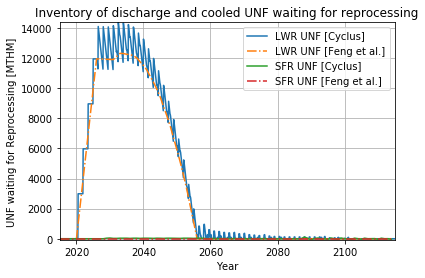
\includegraphics[scale=0.7]{./images/results_18/waiting_monthly.png}
	\end{center}
	\caption{Inventory of discharged and cooled \gls{UNF} waiting for reprocessing.}
	\label{fig:waiting_monthly}
\end{figure}


Figure \ref{fig:rep} shows the reprocessing throughput, which oscillates around
the benchmark solution. No oscillation exists from 2030 to 2055 because the
\gls{LWR} \gls{UNF} reprocessing plant throughput peaks at 2,000 tons per year.

\begin{figure}[htbp!]
	\begin{center}
		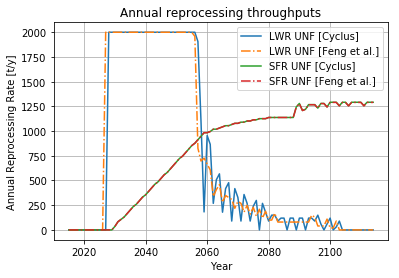
\includegraphics[scale=0.7]{./images/results_18/rep.png}
	\end{center}
	\caption{Annual reprocessing throughputs.}
	\label{fig:rep}
\end{figure}


Figure \ref{fig:tru} shows the inventory of unused \gls{TRU} recovered from \gls{UNF}.
The \Cyclus results follow the benchmark solutions closely. However,
the larger \gls{SFR} core size in Cyclus causes \Cyclus results to be 1.07\% smaller than the benchmark results,
since more \gls{TRU} is used to
start up the newly deployed \glspl{SFR}.

\begin{figure}[htbp!]
	\begin{center}
		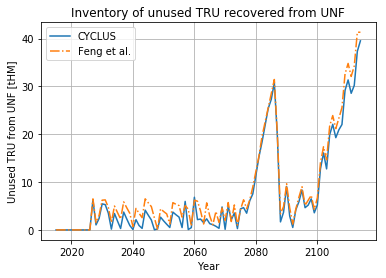
\includegraphics[scale=0.7]{./images/results_18/tru.png}
	\end{center}
	\caption{Inventory of unused \gls{TRU} recovered from \gls{UNF}.}
	\label{fig:tru}
\end{figure}

\FloatBarrier

\section{Discussion}

We verified \Cyclus with results from an established
verification study and saw good agreement
in a transition scenario.

Throughout this work, two major differences were identified
that led to the deviation
of \Cyclus results from that of the benchmark solution. First,
the \Cycamore reactor depletes only half of its core
when decommissioned. Second, \Cyclus, unlike other
codes examined in the benchmark (except ORION), fully resolves
discrete batches for fuel discharge.
We resolve the first discrepancy by changing one line in the Cycamore module
source code.

This study proves that \Cyclus is a capable tool for modeling
fuel cycle transition scenarios.

\FloatBarrier



\chapter{French \gls{NFC} Transition Scenario with \gls{EU} Regional Analysis}

The stated long term plan for nuclear deployment in France targets a technology 
transition to \glspl{SFR} \cite{cne2_reports_2015}. However, the current inventory of French \gls{UNF} 
is insufficient to fuel that transition without building new \glspl{LWR} \cite{carre_overview_2009}.

If instead, France accepted 
\gls{UNF} from other \gls{EU} nations and used it to produce \gls{MOX} for new \glspl{SFR},
the \gls{MOX} created will fuel a French transition to an \gls{SFR} fleet
and allow France to avoid building additional \glspl{LWR}.

To simulate this cooperative scenario, I simulated the entire \gls{EU} region
and all its nuclear reactor operating history and \gls{UNF} accumulation up to the
nearest foreseeable future. Then, France would take as much \gls{UNF} it needs
to transition into a fully \gls{SFR} fleet without building additional \glspl{LWR}.

This chapter includes the results for a French \gls{NFC} transition
scenario from a \gls{LWR} fleet to a fully \gls{SFR} fleet by
taking other \gls{EU} nations' \gls{UNF}.


\subsection{\gls{EU} Deployment Schedule}

The historic \gls{EU} deployment schedule and operation history 
are generated using the \texttt{write\_input.py}
module (described in section \ref{sec:writeinput}).

Projections of future reactor deployment in this simulation are based on
assessment of analyses from references, for instance \gls{PRIS}, for reactors planned
for construction \cite{iaea_nuclear_2017}, the World Nuclear Association
\cite{world_nuclear_association_nuclear_2017}, and literature concerning the future of
nuclear power in a global \cite{joskow_future_2012} and European context
\cite{hatch_politics_2015}.  Existing projections extend to 2050.

\Cref{tab:eu_deployment} lists the reactors that are currently  planned or
under construction in the \gls{EU}. In the simulation, all  planned constructions are completed 
without delay or failure and reach a lifetime of 60 years.  

\pagebreak
\begin{table}[h]
    \centering
    \caption {Power reactors under construction and planned. Replicated from \cite{world_nuclear_association_nuclear_2017}.}
    \label{tab:eu_deployment}
    \begin{tabular}{ccccr}
        \hline
        \textbf{Exp. Operational }&\textbf{Country} &\textbf{Reactor} & \textbf{Type} & \textbf{Gross \gls{MWe}}\\
        \hline
        2018 & Slovakia  & Mochovce 3 & PWR & 440\\
        2018 & Slovakia & Mochovce 4 & PWR & 440 \\
        2018 & France & Flamanville 3 & PWR & 1600 \\
        2018 & Finland & Olkilouto 3 & PWR & 1720 \\
        2019 & Romania & Cernavoda 3 & PHWR & 720 \\
        2020 & Romania & Cernavoda 4 & PHWR & 720 \\
        2024 & Finland & Hanhikivi & VVER1200 & 1200 \\
        2024 & Hungary & Paks 5 & VVER1200 & 1200 \\
        2025 & Hungary & Paks 6 & VVER1200 & 1200 \\
        2025 & Bulgaria & Kozloduy 7 & \footnotemark AP1000 & 950 \\
        2026 & UK & Hinkley Point C1 & EPR & 1670 \\
        2027 & UK & Hinkley Point C2 & EPR & 1670 \\
        2029 & Poland & Choczewo & N/A & 3000 \\
        2035 & Poland & N/A & N/A & 3000 \\
        2035 & Czech Rep & Dukovany 5 & N/A & 1200 \\
        2035 & Czech Rep & Temelin 3 & AP1000 & 1200 \\
        2040 & Czech Rep & Temelin 4 & AP1000 & 1200 \\
        \hline
    \end{tabular}
\end{table}

    \footnotetext{The fate of many planned reactors is uncertain. The proposed reactor types
              are also unclear. The ones marked `N/A' for type are assumed to the \glspl{PWR}
              in the simulation.}
\FloatBarrier

For each \gls{EU} nation, we categorize the growth trajectory from
``Aggressive Growth'' to ``Aggressive Shutdown''. ``Aggressive growth'' is
characterized by a rigorous expansion of nuclear power, while
``Aggressive Shutdown'' is characterized as a transition to rapidly
de-nuclearize the nation's electric grid. We categorize each nation's growth 
trajectory into five degrees depending on G, the growth trajectory metric:

 \[
 G = \left\{\begin{array}{ll}
 \text{Aggressive Growth}, & \text{for } G \geq 2\\
 \text{Modest Growth}, & \text{for } 1.2 \leq G < 2\\
 \text{Maintanence}, & \text{for } 0.8 \leq G < 1.2 \\
 \text{Modest Reduction}, & \text{for } 0.5 \leq G< 0.8\\
 \text{Aggressive Reduction}, & \text{for } G \leq 0.5
 \end{array}\right\} = \frac{C_{2040}}{C_{2017}}\\\\
 \]
 \[
  G = \text{Growth Trajectory  } [-] 
 \]
 \[
 C_{i} = \text{Nuclear Capacity in Year i  } [\gls{MWe}].
 \]

The growth trajectory and specific plan of each nation in the \gls{EU} 
is listed in Table \ref{tab:eu_growth}.  

\begin{table}[h]
    \centering
    \caption{Projected nuclear power strategies of \gls{EU} nations \cite{world_nuclear_association_nuclear_2017}}
        \begin{tabular}{lll}
            \hline 
                    \textbf{Nation} & \textbf{Growth Trajectory} & \textbf{Specific Plan }\\
                    \hline
                    UK & Aggressive Growth & {\small  13 units (17,900 \gls{MWe}) by 2030.}\\
                    Poland & Aggressive Growth &  {\small Additional 6,000 \gls{MWe} by 2035.}\\
                    Hungary & Aggressive Growth &  {\small Additional 2,400 \gls{MWe} by 2025.} \\ 
                    Finland & Modest Growth &  {\small Additional 2,920 \gls{MWe} by 2024.}\\
                    Slovakia & Modest Growth & {\small Additional 942 \gls{MWe} by 2025.}\\
                    Bulgaria & Modest Growth &  {\small Additional 1,000 \gls{MWe} by 2035.} \\
                    Romania & Modest Growth &  {\small Additional 1,440 \gls{MWe} by 2020.} \\
                    Czech Rep. & Modest Growth & {\small  Additional 2,400 \gls{MWe} by 2035.}\\
                    France & Modest Reduction & {\small No expansion or early shutdown.}\\
                    Slovenia & Modest Reduction & {\small No expansion or early shutdown.}\\
                    Netherlands & Modest Reduction & {\small No expansion or early shutdown.}\\
                    Lithuania & Modest Reduction & {\small No expansion or early shutdown.}\\
                    Spain & Modest Reduction &  {\small No expansion or early shutdown.} \\
                    Italy & Modest Reduction & {\small No expansion or early shutdown. }\\
                    Belgium & Aggressive Reduction & All shut down 2025.\\
                    Sweden & Aggressive Reduction & All shut down 2050.\\
                    Germany & Aggressive Reduction & All shut down by 2022.\\
                    \hline
                    
        \end{tabular}
  \label{tab:eu_growth}
\end{table}
\FloatBarrier


Using this categorization to drive facility deployment, the simulation captures 
regional differences in reactor power capacity and \gls{UNF} production as a 
function of time. Accordingly, \cref{fig:eu_pow} shows the resulting simulated 
installed capacity in \gls{EU} nations.  Sudden capacity reductions seen in the 
2040s result from end-of-license reactor retirements and nuclear phaseout plans 
in nations such as Germany and Belgium.  

\begin{figure}[htbp!]
    \begin{center}
        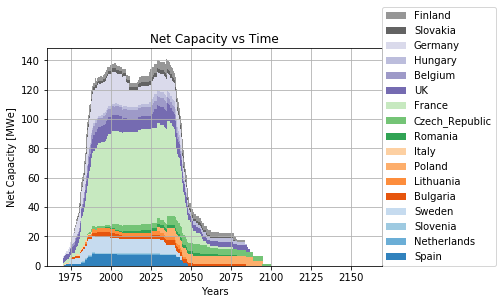
\includegraphics[scale=0.6]{./images/eu_future/power_plot.png}
    \end{center}
    \caption{Installed nuclear capacity in the EU is distinguished by \texttt{Region}s in \Cyclus.}
    \label{fig:eu_pow}
\end{figure}


\subsection{French \gls{SFR} Deployment Schedule}

\Cref{fig:sfr_num}
shows
the French transition to \glspl{SFR} modeled in this simulation.
Historically aggressive growth of nuclear in the 1980s leads to a substantial 
shutdown of nuclear in the 2040s, which, in the simulation, are replaced by new 
\glspl{SFR}. The net capacity is kept constant at 66 GWe.

\begin{figure}[htbp!]
        \begin{center}
                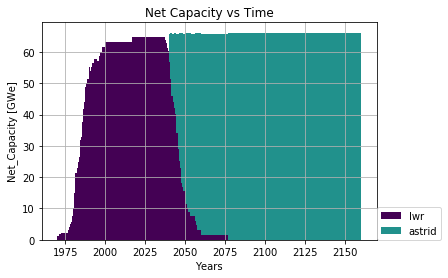
\includegraphics[scale=0.6]{./images/french-transition/power_plot.png}
        \end{center}
        \caption{The potential French transition from \glspl{LWR} to 
                \glspl{SFR} when assisted by \gls{UNF} from other \gls{EU} 
        nations.}
        \label{fig:sfr_num}
\end{figure}

\Cref{fig:french_dep} shows the deployment required to support the transition in 
\cref{fig:sfr_num}. France must build four reactors per year, on average, to 
make up for the end-of-license decommissioning of power plants built in the 1980s and 1990s.  The second period of aggressive building occurs when the first generation of \glspl{SFR} decommission after 80 years. Starting in 2040, France deploys 600-\gls{MWe} \glspl{SFR} to make up for 
decommissioned French \gls{LWR} capacity. This results in an installed 
\gls{SFR} 
capacity of 66,000 \gls{MWe} by 2078 when the final \gls{LWR} is 
decommissioned. 



\begin{figure}[htbp!]
    \begin{center}
        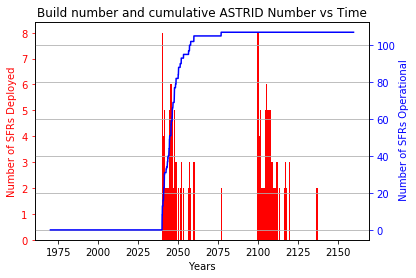
\includegraphics[scale=0.6]{./images/french-transition/sfr_deploy.png}
    \end{center}
    \caption{The deployment of \glspl{SFR} in France is characterized by a period of
    aggressive building.}
    \label{fig:french_dep}
\end{figure}


Finally, \Cref{fig:tot_dep} shows the total deployment scheme we simulated.  
The French transition to \glspl{SFR} couples with the historical and projected 
operation of \gls{EU} reactors.  The steep transition from 2040 to 2060 
reflects the scheduled decommissioning of reactors built in the 1975-2000 era 
of aggressive nuclear growth in France.

\begin{figure}[htbp!]
    \begin{center}
        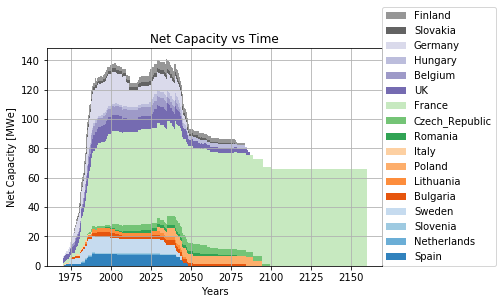
\includegraphics[scale=0.6]{./images/eu_future/onesim.png}
    \end{center}
    \caption{The total deployment scheme we simulated relies on \gls{UNF} 
    collaboration among nations.} 
    \label{fig:tot_dep}
\end{figure}

These figures reflect that, for the given assumptions, bursts of construction
are necessary to maintain capacity.  In reality, a construction rate of five 
reactors every year is ambitious, but might have the advantage of
larger scale production of components and more modular assembly and construction if major components can mostly be built off site.

This analysis establishes a multi-national material flow and demonstrates that, if such an aggressive deployment scheme took place, the \glspl{SFR} would have enough fuel.

\subsection{Material Flow}

The fuel cycle is represented by a series of facility agents whose material 
flow is illustrated in figure \ref{diag:fc}, along with
the \Cyclus archetypes that were used to model each facility.
In this diagram, \gls{MOX} Reactors include both French \glspl{PWR} and 
\glspl{SFR}.

% Define block styles
\tikzstyle{decision} = [diamond, draw, fill=blue!20, 
text width=4.5em, text badly centered, node distance=3cm, inner sep=0pt]
\tikzstyle{block} = [rectangle, draw, fill=blue!20, 
text width=5em, text centered, rounded corners, minimum height=4em]
\tikzstyle{line} = [draw, -latex']
\tikzstyle{cloud} = [draw, ellipse,fill=red!20, node distance=3cm,
minimum height=2em]


\begin{figure}
	\centering
	\scalebox{0.6}{
		\begin{tikzpicture}[align=center, node distance = 3cm and 3cm, auto]
		% Place nodes
		\node [block] (sr) {Mine (\texttt{SOURCE})};
		\node [cloud, below of=sr] (nu) {Nat U};
		\node [block, below of=nu] (enr) {Enrichment ({\footnotesize \texttt{ENRICHMENT}})};
		\node [cloud, below of=enr] (uox) {\acrshort{UOX}};
		\node [block, below of=uox] (lwr) {\gls{LWR} (\texttt{REACTOR})};
		\node [cloud, right of=lwr] (snf) {\gls{UNF}};
		\node [block, right of=snf] (pool) {Pool (\texttt{Storage})};
		\node [cloud, left of=lwr] (tl2) {Dep U};
		\node [cloud, right of=enr] (tl) {Dep U};
		\node [block, right of=tl] (sk) {Repository (\texttt{SINK})};
		\node [cloud, below of=sk] (cunf) {Cooled \gls{UNF}};
		\node [cloud, below of=pool] (cunf2) {Cooled \gls{UNF}};
		\node [block, below of=snf] (rep) {{\small Reprocessing ({\footnotesize \texttt{SEPARATIONS}})}};
		\node [cloud, below of=rep] (u) {Sep. U} ;
		\node [cloud, left of=rep] (pu) {Sep. Pu};
		\node [block, left of=pu] (mix) {Fabrication (\texttt{MIXER})};
		\node [cloud, below of=mix] (mox) {\gls{MOX}};
		\node [block, below of=mox] (mxr) {\gls{MOX} Reactors 
			(\texttt{REACTOR})};
		\node [cloud, right of= mxr] (snmox) {Spent \gls{MOX}};
		
		\draw[->, thick] (sr) -- (nu);
		\draw[->, thick] (nu) -- (enr);
		\draw[->, thick] (enr) -- (tl);
		\draw[->, thick] (enr) -- (tl2);
		\draw[->, thick] (tl) -- (sk);
		\draw[->, thick] (tl2) -- (mix);
		\draw[->, thick] (enr) -- (uox);
		\draw[->, thick] (uox) -- (lwr);
		\draw[->, thick] (lwr) -- (snf);
		
		\draw[->, thick] (lwr) -- (snf);
		\draw[->, thick] (snf) -- (pool);
		\draw[->, thick] (pool) -- (cunf);
		\draw[->, thick] (pool) -- (cunf2);
		\draw[->, thick] (cunf) -- (sk);
		\draw[->, thick] (cunf2) -- (rep);
		
		\draw[->, thick] (rep) -- (u);
		\draw[->, thick] (rep) -- (pu);
		\draw[->, thick] (pu) -- (mix);
		\draw[->, thick] (mix) -- (mox);
		\draw[->, thick] (mox) -- (mxr);
		\draw[->, thick] (mxr) -- (snmox);
		\draw[->, thick] (snmox) -- (rep);
		
		\end{tikzpicture}
		
	}
	\caption{Fuel cycle facilities (blue boxes) represented by 
		\Cyclus archetypes (in parentheses) pass materials (red 
		ovals) around the simulation.} 
	\label{diag:fc}
\end{figure}

A mine facility provides natural uranium, which is enriched by an enrichment
facility to produce \gls{UOX}. Enrichment wastes (tails) are disposed of to a 
sink facility representing ultimate disposal. The enriched \gls{UOX} fuels
the \glspl{LWR} which in turn produce spent \gls{UOX}. The used fuel
is sent to a wet storage facility for a minimum of 72 months. \cite{carre_overview_2009}.

The cooled fuel is then reprocessed to separate plutonium and uranium,
or sent to the repository.
The plutonium mixed with depleted uranium (tails) makes \gls{MOX} (Both for
French \glspl{LWR} and \glspl{ASTRID}).
Reprocessed uranium is unused and stockpiled. Uranium is reprocessed
in order to separate the raffinate (minor actinides and fission products)
from usable material. Though neglected in this work, reprocessed
uranium may substitute depleted uranium for \gls{MOX} production. In the
simulations, sufficient depleted uranium existed that the complication of
preparing reprocessed uranium for incorporation into reactor fuel
was not included. However, further in the future where the depleted
uranium inventory drains, reprocessed uranium (or, natural uranium) will need to be utilized. 

\FloatBarrier
\subsection{Scenario Specification}

The scenario specifications defining the simulations presented in this work 
are listed in table \ref{tab:gen}.
The reprocessing and \gls{MOX} fabrication capacity in France
prior to 2020 is modeled after the 
French La Hague and MELOX sites \cite{schneider_spent_2008, hugelmann_melox_1999}.


\begin{table}[h]
    \centering
    \caption{Simulation Specifications}
    \begin{tabularx}{\linewidth}{bss}
        \hline
        \textbf{Specification} &\textbf{ Value} & \textbf{Units}\\
        \hline
        Simulation Starts & 1970 & year\\
        Simulation Ends & 2160 & year\\ 
        Production of \gls{ASTRID} fuel begins & 2020 & year\\
        \glspl{SFR} become available & 2040 & year\\
        Reprocessed uranium usage &  Not used anywhere & -\\
        Minimum \gls{UNF} cooling time  & 36  & months\\
        Separation efficiency of U and Pu & 99.8 & \% \\
        Reprocessing streams & Pu and U & - \\
        Reprocessing capacity before 2020 & 91.6 \cite{schneider_spent_2008} & $\frac{\text{metric tons of \gls{UNF}}}{month}$  \\
        Reprocessing capacity after 2020 & 183.2 & $\frac{\text{metric tons of \gls{UNF}}}{month}$\\
        \gls{LWR} \gls{MOX} fabrication throughput & 16.25 \cite{hugelmann_melox_1999} & $\frac{\text{metric tons of \gls{MOX}}}{month}$\\
        \gls{ASTRID} \gls{MOX} fabrication throughput & No limit ($\infty$) & $\frac{\text{metric tons of \gls{MOX}}}{month}$ \\
        \gls{LWR} \gls{MOX} recycling  &  Not reprocessed & - \\
        \gls{ASTRID} \gls{MOX} recycling & $\infty$-pass & - \\
        \hline
    \end{tabularx}
    \label{tab:gen}
\end{table}



\pagebreak

\section{Reactor Specifications}
Three major reactors are used in the simulation, \gls{PWR}, \gls{BWR}, and ASTRID-type \gls{SFR} reactors.
The \gls{PWR} and \gls{BWR} specifications are determined using the linear core size model,
as explained in section \ref{sec:writeinput}. The ASTRID-type \gls{SFR} specification
is obtained from varaine et al \cite{varaine_pre-conceptual_2012}.

\begin{table}[h]
    \centering
    \caption{Baseline \gls{LWR} and \gls{ASTRID} simulation specifications.}
    \begin{tabular}{lrrr}
        \hline
        \textbf{Specification} & \textbf{\gls{PWR} \cite{sutharshan_ap1000tm_2011}} & \textbf{\gls{BWR} \cite{hinds_next-generation_2006}} & \textbf{\gls{SFR}} \cite{varaine_pre-conceptual_2012}\\
        \hline
                Lifetime [y] \tablefootnote{The simulated reactor lifetime reaches the licensed lifetime unless 
        the reactor is shut down prematurely.} & 60 & 60 & 80 \\
                Cycle Time [mos.]& 18 & 18 & 12\\ 
                Refueling Outage [mos.]& 2 & 2  & 2\\
                Rated Power [\gls{MWe}] & 1110 & 1000 & 600\\
                Assembly mass [kg] & 446 & 180 & -- \\
                Batch mass [kg] & -- & -- & 5,568\\
                Discharge Burnup [GWd/tHM] & 51 & 51 & 105 \\
                Assemblies per core \tablefootnote{Number of assemblies and corresponding \gls{LWR} core 
        masses are reported for a 1100-\gls{MWe} core. Reactors with different core  
        powers are modeled with a linear mass assumption.} & 157  & 764 & -- \\

                Batches per core & 3 & 3 & 4\\
        Initial Fissile Loading [t] & 3.1  $^{235}$U & 4.2  $^{235}$U & 4.9 Pu \\
                Fuel & \gls{UOX} or \gls{MOX} & \gls{UOX} & \gls{MOX} \\
        \hline
    \end{tabular}
        
    \label{tab:reactor-specs}

    \end{table}


\subsection{Material Definitions}
Depletion calculations of the nuclear fuel are recipe-based, such that a fresh 
and used fuel recipe is defined for each reactor type.
For the compositions of the used fuel, a reference depletion calculation
from ORIGEN is used (see \cref{tab:comp}). ORIGEN calculates buildup,
 decay, and processing of radioactive materials
\cite{parks_overview_1992}. This recipe has also been used for repository performance modeling \cite{wilson_adoption_2009}.

\begin{table}[h]
    \centering
    \caption{Fresh fuel compositions in the simulation \cite{wilson_adoption_2009, varaine_pre-conceptual_2012}.}
%   \scalebox{0.86}{
        \begin{tabular}{lrrr}
            \hline
             & \multicolumn{3}{c}{ Composition [\%]} \\
            Recipe & U-235  & U-238  & Pu \\ 
            \hline
            Fresh \gls{UOX} Fuel & 3.1 & 96.9 & -   \\ 
            Fresh \gls{LWR} \gls{MOX} Fuel & 0.2 & 90.7 & 9.1 \\ 
            Fresh \gls{ASTRID} Fuel & 0.2 & 77.7 & 22 \\
            \hline
        \end{tabular}
        
        \label{tab:sim_result}
\end {table}



\subsection{Results - Transition Scenario}
This section displays the simulation results if France utilized
\gls{UNF} from other \gls{EU} nations to fuel the transition into a fully
\glspl{ASTRID} fleet.

\subsubsection{Nuclear Fuel Material Inventory}
\Cref{tab:sim_result1} 
lists \gls{EU} material inventory in 2050.
The materials continue to accumulate after 2050, but the
\gls{UNF} France receives before 2050 is most impactful for the
feasibility of the transition. Note that \cref{tab:sim_result1} 
distinguishes the
\gls{UOX} in the simulation either stored or reprocessed to create \gls{MOX}.


\begin{table}[h]
    \centering
        \caption{\gls{EU} nuclear material inventory in 2050.}
\begin{tabularx}{\textwidth}{XrX}
            \hline
                        \textbf{Category} & \textbf{Value} & Specifics \\
                                          & \textbf{[MTHM]} & \\ \hline
                        UOX Loaded  & 161,894 & UOX used in EU (minus France) reactors 1970-2050\\ 
            MOX Loaded  & 6,945  & MOX used in French reactors 1970-2050\\
                        Available used UOX (EU)  & 95,193  & Used EU (minus France) 
                                UOX in storage for future ASTRID MOX 
                                production\\
                        Available used UOX (France) & 
                                10,029  & Used French UOX stored for 
                                future ASTRID MOX production. \\
                                Reprocessed UOX (France) & 53,590 & Used French UOX already reprocessed for the production of LWR MOX \\
            Tails  & 980,294  & (Tails generated) $-$ (Tails used for production of LWR MOX) \\ 
            Natural U Used  & 1,142,189  & \\ \hline
        \end{tabularx}
        
        \label{tab:sim_result1}
\end {table}
\FloatBarrier


Figures \ref{fig:eu_tail} and \ref{fig:eu_snf} show the 
accumulation of tails and used fuel over time in the \gls{EU}.
Tails accumulate as a by-product of uranium enrichment. For every
ton of \gls{UOX} fuel, about nine times of tails is produced. 
Spent fuel is discharged from reactors every refueling period.
The entire core is discharged when the reactor decommissions.
A total of about $1,000,000$ MTHM of tails and $100,000$ MTHM of
\gls{UNF} have accumulated by 2050.
Figure \ref{fig:eu_fuel} shows the amount of fuel used in the \gls{EU}. The 
tails mass accumulation rate is fairly steady, with peaks occurring when new 
reactors are deployed.
In \cref{fig:eu_snf}, the peaks are caused by reactor decommissioning which 
triggers all the batches in the final reactor core to be sent to the repository.

\begin{figure}[htbp!]
    \begin{center}
        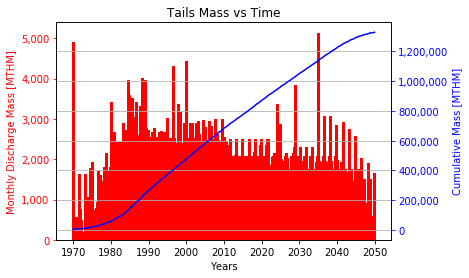
\includegraphics[scale=0.7]{./images/eu_future/tails.png}
    \end{center}
        \caption{Simulated accumulation of tails in the \gls{EU} is shown as a function of time.}
    \label{fig:eu_tail}
\end{figure}

\begin{figure}[htbp!]
    \begin{center}
        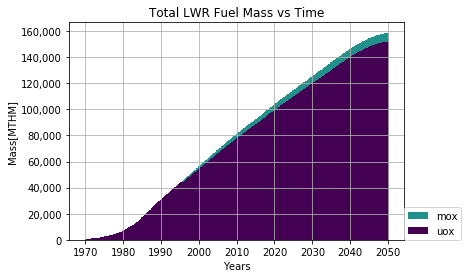
\includegraphics[scale=0.7]{./images/eu_future/total_fuel.png}
    \end{center}
\caption{Simulated total \gls{EU} fuel useage is shown as a function of time.}
    \label{fig:eu_fuel}
\end{figure}


\begin{figure}[htbp!]
    \begin{center}
            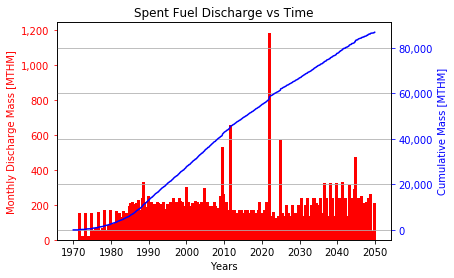
\includegraphics[scale=0.7]{./images/eu_future/snf_discharge.png}
    \end{center}
        \caption{Simulated \gls{EU} \gls{UNF} accumulation and discharge is 
shown as a function of time.}
    \label{fig:eu_snf}
\end{figure}


\subsubsection{French \gls{SFR} Deployment}
\FloatBarrier

Reprocessing the \gls{UNF} collected from all EU nations can provide the 
initial cores for approximately 180 \glspl{SFR}. Table \ref{tab:pu} lists the 
isotope, mass fraction, and quantity of plutonium that can be obtained from the 
2050 \gls{UNF} inventory.  With the \gls{SFR} breeding ratio above one, France 
can transition into a fully \gls{SFR} fleet without extra construction of 
\glspl{LWR}. 

\begin{table}[h]
    \centering
    \caption{Plutonium in the \gls{UNF} inventory.}
    \begin{tabular}{lrr}
        \hline
        \textbf{Isotope} & \textbf{Mass Fraction in Used Fuel [\%]} & \textbf{Quantity [t]} \\ \hline
        Pu238 & 0.0111 & 10.52 \\ 
        Pu239 & 0.518 & 545.05 \\ 
        Pu240 & 0.232 & 244.11 \\ 
        Pu241 & 0.126 & 132.58 \\ 
        Pu242 & 0.0487 & 51.24 \\ \hline
        \textbf{Total} & \textbf{0.9358} & \textbf{983.52} \\ \hline
    \end{tabular}
    
    \label{tab:pu}
\end{table}

From Varaine et al. \cite{varaine_pre-conceptual_2012}, a French
ASTRID-type 600\gls{MWe} \gls{SFR} consumes $1.225$ metric tons of
plutonium a year, with an initial plutonium loading of $4.9$ metric tons. 
Thus, the number of \glspl{SFR} that can be loaded with the reprocessed
plutonium from \gls{UNF} can be estimated to be 200, assuming adequate 
reprocessing and fabrication capacity as well as abundant depleted uranium 
supply.
 
Used \gls{MOX} from an ASTRID reactor is 23.95\% plutonium
in this simulation (see \cref{tab:comp}), whereas fresh \gls{MOX} is 22\% plutonium.
The plutonium breeding ratio in this simulation is thus assumed to be
$\approx 1.08$.

\Cref{fig:fuel} shows \gls{MOX} loaded in the \glspl{SFR} per month.  The plot 
has peaks during a period of aggressive deployment of \glspl{SFR} followed by 
an equilibrium at 100 \gls{MTHM}. The peaks reoccur with the deployment of the 
second generation of \glspl{SFR}.  The spikes are due to initial fuel demand 
correspoding to these new deployments.  The initial cores loaded into new 
\glspl{SFR} rely on the \gls{MOX} created from legacy \gls{UNF}. Once the 
deployed \glspl{SFR} create enough extra plutonium, the legacy \gls{UNF} is no 
longer used. Notably, this switch from a less preferred fuel origin to a more 
preferred fuel origin is handled automatically within \Cyclus via user-defined preferences 
within its dynamic resource exchange algorithm \cite{gidden_methodology_2016}.


\begin{figure}[htbp!]
    \begin{center}
        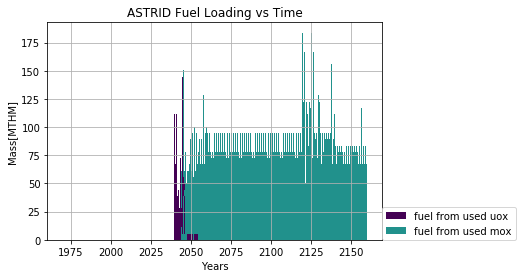
\includegraphics[width=0.7\textwidth]{./images/french-transition/where_fuel.png}
    \end{center}
    \caption{Fuel loaded into \glspl{SFR} was simulated in discrete 
        batches.}
    \label{fig:fuel}
\end{figure}

\Cref{fig:pu_no_cum} shows the separated plutonium discharge per month from the reprocessing plant. The plutonium outflux does not precisely follow the fuel demand because \Cyclus agents have material buffers that store commodity fuel for later usage. The reprocessed plutonium from legacy \gls{UNF} is stored for the initial loading of \glspl{SFR}.  Plutonium separated from legacy \gls{UNF} meets plutonium demans sufficiently to reduce the reprocessing demand for the first aggressive deployment of \glspl{SFR}.  The plutonium from reprocessing legacy fuel is a flat rectangle because the reprocessing throughput was set to 183.2 $\frac{\gls{MTHM}}{month}$ to avoid reprocessing all the legacy in one timestep. 
 

\begin{figure}[htbp!]
    \begin{center}
        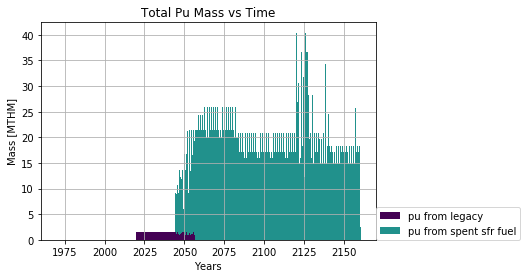
\includegraphics[scale=0.7]{./images/french-transition/pu.png}
    \end{center}
    \caption{The separated plutonium discharge from the reprocessing plant 
        in $\frac{\mbox{MTHM}}{\mbox{month}}$.}
    \label{fig:pu_no_cum}
\end{figure}

 \Cref{tab:sfr_sim_result} lists metrics obtained from the second simulation.

\begin{table}[h]
    \centering
    \caption {In the French transition to \glspl{SFR},
                  the total legacy \gls{UNF} reprocessed is the 
                                  amount of \gls{UNF} France needs 
                  for a transition into a fully \gls{SFR} fleet. 
                                  %The tails used is around ninth of the original tails inventory from the previous simulation.
                                  %KDH note: What does this mean?
                                  %thought there was only one simulation. . . 
                          }
    \scalebox{0.86}{
        \begin{tabular}{llr}
            \hline
            \textbf{Category} & \textbf{Unit} & \textbf{Value}  \\ \hline
            Total \gls{ASTRID} MOX used & MTHM & 63,447  \\ 
            \textbf{Average UOX Reprocessing} & MTHM/month & \textbf{123.27} \\
            \textbf{Average Total Reprocessing} & MTHM/month & \textbf{63.23} \\
            \textbf{Average Fuel Fabrication} & MTHM/month & \textbf{74.31} \\
            Total \glspl{SFR} Deployed & & 220 \\ 
            Total Plutonium Reprocessed & MTHM & 14,831 \\ 
            Total \gls{ASTRID} fuel from UOX Waste & MTHM & 2,895  \\ 
            Total \gls{ASTRID} fuel from MOX Waste & MTHM  & 60,552 \\ 
            Total Tails used & MTHM & 49,488 \\ 
            \textbf{Total legacy UNF reprocessed} & MTHM & \textbf{53,595} \\ 
            Total Reprocessed Uranium Stockpile & MTHM & 159,383 \\ 
            Total Raffinate & MTHM & 24,789 \\ \hline
        \end{tabular}}
        
        \label{tab:sfr_sim_result}
\end {table}


These results demonstrate that despite the large amount of initial plutonium that has to be reprocessed
prior to \gls{ASTRID} deployment, the 20 years (2020-2040) of 
\gls{ASTRID} fuel preparation
allows a reasonable level of average
\gls{UOX} reprocessing capacity demand. \gls{UOX} reprocessing continues 
until 2057, when the \gls{ASTRID} spent fuel can supply the plutonium
for its own fuel.

\subsubsection{Conclusion}

France can transition into
a fully \gls{SFR} fleet with installed capacity of 66,000 \gls{MWe} without
building additional \glspl{LWR}
if France receives \gls{UNF} from other \gls{EU} nations.
Supporting the \gls{SFR} fleet requires an average 
reprocessing capacity of 73.27 \gls{MTHM} per month,
and an average fabrication capacity of 45.29 \gls{MTHM} per month.

Since most \gls{EU} nations do not have an operating \gls{UNF}
repository or a management plan, they have a strong incentive
to send their \gls{UNF} to France. In particular, the nations
planning aggressive nuclear reduction will be able phase out nuclear
without constructing a permanent repository. France has an
incentive to take this fuel, since recycling used fuel from
other nations will allow France to meet their MOX demand
without new construction of \glspl{LWR}.

\Cref{tab:which_send} lists \gls{EU} nations and their \gls{UNF} inventory
in 2050. We analyzed a strategy in which 
the nations reducing their nuclear fleet send their \gls{UNF} to France.
The sum of \gls{UNF} from Italy, Slovenia, Belgium, Spain and Germany
provides enough \gls{UNF} for the simulated transition ($\approx 54,000$ MTHM). 
These nations are shown in bold in \cref{tab:which_send}.
Sweden is not considered because of its concrete waste management plan.


\begin{table}[h]
    \centering
    \caption {\gls{EU} nations and their respective \gls{UNF} inventory.} 
                \begin{tabularx}{\textwidth}{llr}
                    \hline 
                    \textbf{Nation} & \textbf{Growth Trajectory} & \small{\textbf{UNF in 2050 [MTHM] }}\\
                    \hline
                    Poland & Aggressive Growth & 1,807\\
                    Hungary & Aggressive Growth & 3,119 \\ 
                    UK & Aggressive Growth & 13,268\\
                    Slovakia & Modest Growth & 2,746\\
                    Bulgaria & Modest Growth & 3,237 \\
                    Czech Rep. & Modest Growth & 4,413\\
                    Finland & Modest Growth &  5,713\\
                    Netherlands & Modest Reduction & 539\\
                    \textbf{Italy} & \textbf{Modest Reduction} & \textbf{583}\\
                    \textbf{Slovenia} & \textbf{Modest Reduction} & \textbf{765}\\
                    \textbf{Lithuania} & \textbf{Modest Reduction} & \textbf{2,644} \\
                    \textbf{Belgium} & \textbf{Aggressive Reduction} & \textbf{6,644}\\
                    \textbf{Spain} & \textbf{Modest Reduction} &  \textbf{9,771} \\
                    \textbf{France} & \textbf{Modest Reduction} & \textbf{9,979} \\
                    Sweden & Aggressive Reduction & 16,035\\
                    \textbf{Germany} & \textbf{Aggressive Reduction} & \textbf{23,868}\\
                    \hline
                \end{tabularx}
    
    \label{tab:which_send}

\end{table}

On the other hand, in these simulations, some complex political and economic factors were not incorporated and various assumptions were present in this scenario. For
example, Germany's current policy is to not reprocess its \gls{LWR} fuel
\cite{topfer_germanys_2011}, and this policy would create a shortage
in the supply of \gls{LWR} \gls{UNF} for \gls{ASTRID} \gls{MOX} production.
Continuation of that German policy would not, however, be incompatible
with a change in \gls{EU} policy that frees \gls{EU} countries from
creating their high level waste repositories, since France could still
agree to take in Germany's \gls{UNF} for direct disposal. The analysis
method described herein could readily be adapted to account for such possibilities. 
The collaborative option explored here may hold value for the \gls{EU} nuclear community,
and may enable France to advance more rapidly into a closed fuel cycle. 
\FloatBarrier


\chapter{United States \gls{NFC} Transition Scenario}
nuThe United States has been the forerunner in nuclear energy, with a currently 
installed nuclear capacity of 99,221 \gls{MWe} \cite{iaea_nuclear_2017}.
With its large capacity and long history of nuclear
energy, the United States has accumulated over $70,000$ \gls{MTHM} of \gls{UNF}.

The challenge with modeling the U.S. transition scenario is that the U.S. does not have
a single nationwide advanced reactor vision, whereas France has a central plan to transition into \gls{ASTRID} reactors \cite{boullis_french_2015, varaine_pre-conceptual_2012}.
Previous analyses of the United States \cite{worrall_utilization_2013, sunny_transition_2015}
 \gls{NFC} transition scenario
assumed transition to fast-spectrum \glspl{SFR}.
However, the fact that the U.S. nuclear reactor fleet
is decided by economic interests (industries), necessitates
exploration of different options, such as transitioning into \glspl{MSR}.

As explained in section \ref{sec:msr}, rising interests in \gls{MSR} designs
led to a proliferation of U.S. corporations aiming to commercialize
\gls{MSR} designs. Given the large interest from industries,
\gls{MSR} designs may someday be commercially deployed in the United
States.


In this chapter, I explore the U.S. transition scenario
from an \gls{LWR} fleet into an \gls{MSR} fleet.

\section{Initial conditions and scenario parameters}

For the French scenario, the \gls{UNF} inventory at the present
time is calculated by simulating the nuclear operational history from 1970.
However, this is unnecessary for the U.S. scenario because a detailed
database exists that describes the U.S. \gls{UNF} inventory up to May of 2013.
The \gls{UNF-STANDARDS} is a comprehensive,
controlled source of \gls{UNF} information, including dry cask attributes, assembly
data, and economic attributes \cite{peterson_unf-st&dards_2017}. The assembly
compositions are calculated using ORIGEN \cite{parks_overview_1992} using the
reported fuel assembly burnups, original enrichment, and assembly design. This database
allows the transition scenario simulation to start from 2013. I imported 
the \gls{UNF} inventory mass and composition in 2013
from \gls{UNF-STANDARDS} and `initiated' the inventory in the simulation
as a \texttt{Source} facility with an inventory of 68,072 MTHM,
the total mass of the \gls{LWR} \gls{UNF} in the \gls{UNF-STANDARDS}.

Furthermore, the U.S. currently has additional uranium resources in the
form of more than $700,000$ MTHM of depleted uranium \cite{office_nuclear_2011},
which is a waste product of enrichment. The depleted uranium inventory
is currently a liability and waste, but can be utilized as fertile material
in a U-Pu fuel cycle. If the U.S. chooses a Th-$^{233}U$ fuel cycle,
additional thorium resources are needed, while with a U-Pu cycle, the
U.S. can use its waste to create fuel.

The U.S. nuclear fleet in 2013 can be extracted from the \gls{PRIS} database.
The same assumption that legacy reactors have a 60-year lifetime is applied
to calculate the remaining lifetime of legacy reactors.
I used \texttt{from\_pris} to generate the expected power capacity
of the current U.S. nuclear from 2013 (shown in figure \ref{fig:us_legacy}).

\begin{figure}[htbp!]
	\begin{center}
		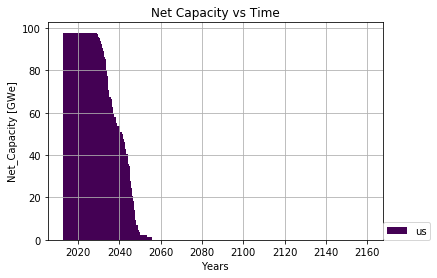
\includegraphics[scale=0.7]{./images/us/legacy_power.png}
	\end{center}
	\caption{Installed nuclear capacity in the United States from 2013.}
	\label{fig:us_legacy}
\end{figure}


\subsection{Energy demand prediction}
A reference for the energy demand prediction is the 
\gls{EIA} Annual Energy Outlook \cite{u.s._eia_annual_2018}.
The 2018 Annual Energy Outlook report predicts an annual electricity demand growth
of 0.9\%. The report also predicts that nuclear
power will either remain static or decrease. The report
predicts that nuclear capacity will decrease from 99 GWe
to 79GWe in 2050, with no new plants beyond 2020.
However, for this work,
I assume that the U.S. nuclear power capacity is kept at
100GWe, and new reactors are deployed to make up for the
decommissioned capacity.

\subsection{\gls{MSR} design and availability}

\gls{MSR} designs can be categorized depending on their operating
neutron spectrum (e.g. fast, thermal), fuel cycle (e.g. Th-$^{233}U$, U-Pu),
and transmutation goals (e.g. breeder, burner). Selection of an \gls{MSR}
design depends on factors like economics, safety, and fuel cycle
considerations. For this work, I choose a fast, U-Pu cycle, burner \gls{MSR} design
named REBUS-3700 \cite{mourogov_potentialities_2006} to deploy for the
transition analysis.

The REBUS-3700 \gls{MSR} design offers five principal
advantages over other \gls{MSR} designs:
\begin{itemize}
	\item Fast spectrum - no need for moderator rods
	\item U-Pu cycle - requires only depleted uranium for supply after initial fuel salt loading
	\item Weakly positive breeding gain (0.03)
	\begin{itemize}
		\item Self-sufficient (no external fissile input)
		\item No surplus fissile material production (stabilizes Pu inventory)
	\end{itemize}
	\item U-\gls{TRU} initial fuel - transmutation of long-lived actinides
	\item Simpler design - no radial / axial blanket
\end{itemize}

The U.S. has a large inventory of \gls{LWR} \gls{UNF} and tails. The benefits
of the REBUS-3700 design aligns with the waste management interest
of the U.S. Reducing final geological repository burden can be
accomplished by:

\begin{itemize}
	\item Reduction of \gls{TRU} inventory by transmutation in the reactor (table \ref{tab:rebus_comp})
	\begin{itemize}
		\item Reduction of long-term decay heat and activity (figure \ref{fig:decay_heat})
		\item More `tailored' waste form design for fission products
	\end{itemize}
	\item Reducing tails inventory
\end{itemize}

Additionally, the REBUS-3700 does not have, at any moment in
operation, separated fissile streams, like other \gls{MSR} designs.
Other \gls{MSR} designs such as the
\gls{MCSFR} design \cite{smith_assessment_1974}
have separated fissile streams, since it separates the bred plutonium from its blanket salt.
The REBUS-3700 only takes in depleted uranium and processes out
fission product groups such as volatile gases and noble metals.
The detailed reprocessing scheme is shown
in table \ref{tab:rebus_reproc}. 
This self-sustained and closed operation increases its non-proliferation
properties.

The initial fuel and equilibrium \gls{TRU} isotopic composition of REBUS-3700 is
shown in table \ref{tab:rebus_comp}. The \gls{TRU} isotopic composition
matches that of the \gls{LWR} \gls{UNF} after 8.5 years of decay (shown
in figure \ref{fig:trutru}).


\begin{figure}[htbp!]
	\begin{center}
		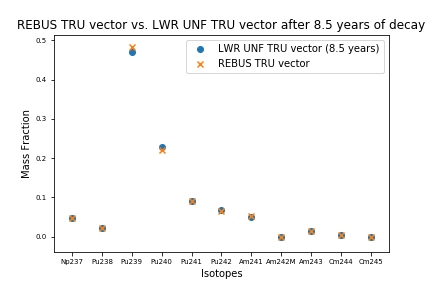
\includegraphics[scale=0.7]{./images/us/trutru.png}
	\end{center}
	\caption{\gls{TRU} vector of REBUS-3700 initial fuel from Mourogov et al. \cite{mourogov_potentialities_2006}
		with \gls{LWR} \gls{UNF} after 51 GWdth/MTHM burnup and 8.5 years of decay}
	\label{fig:trutru}
\end{figure}


\begin{table}[h]
	\centering
	\caption{Initial and equilibrium \gls{TRU} isotopic composition from Mourogov et al. \cite{mourogov_potentialities_2006}.}
	\label{tab:rebus_comp}
	\begin{tabularx}{\textwidth}{lll}
		\hline
		Isotope & Beginning of Life & Equilibrium (\textasciitilde 6500 \gls{EFPD}) \\
		\hline
		$^{237} Np$ / $^{239} Np$ &  4.80 / 0.00 & 0.65 / 0.07 \\
		$^{238} Pu$ / $^{239} Pu$ & 2.13 / 48.33  & 2.23 / 58.02  \\
		$^{240} Pu$ / $^{241} Pu$ / $^{242} Pu$ & 22.17 / 9.05 / 6.38 & 27.63 / 3.35 / 4.05 \\
		$^{241} Am$ / $^{242m} Am$ / $^{243} Am$ &5.17 / 0.01 / 1.48 & 1.50 / 0.12 / 1.05 \\
		$^{242} Cm$ / $^{243} Cm$  & 0.0 /0.0  & 0.07 / 0.01  \\
		$^{244} Cm$ / $^{245} Cm$ / $^{246} Cm$ & 0.43 / 0.04 / 0.00 & 1.02 / 0.19 / 0.05 \\
		Equivalent enrichment, \% & 10.1 & 11.0 \\
		\gls{TRU} fraction in heavy atoms, \% & 15.6 & 15.9 \\
		\hline
	\end{tabularx}
\end{table}


\begin{table}[h]
	\centering
	\caption{Reprocessing scheme for REBUS-3700}
	\label{tab:rebus_reproc}
	\begin{tabular}{lll}
		\hline
		Group & Elements & Reprocessing Time (s) \\
		\hline
		Volatile Gases & Kr, Xe, Ar, Ne, H, N, O, Rn & 30 \\
		Noble Metals & \shortstack{Se, Nb, Mo, Tc, Ru, Rh,\\ Pd, Ag, Sb, Te, Zr, Cd, In, Sn} & 30 \\
		Rare Earths & \shortstack{Y, La, Ce, Pr, Nd, Pm, Sm, Gd, \\ Eu, Dy, Ho, Er, Tb, Ga, Ge, As, Zn} & 259,200 \\
		\hline
	\end{tabular}
\end{table}



\section{U.S. deployment schedule}

As shown in figure \ref{fig:us_legacy}, the U.S. will
undergo a profound loss of nuclear capacity from 2030, under the
assumption that U.S. reactors have a lifetime of 60 years.

Since it is unlikely that \glspl{MSR} are ready for
commercial deployment in 2020, I deploy \glspl{LWR} (AP 1000 design \cite{sutharshan_ap1000tm_2011})
to make up for the decommissioned capacity in the simulation. After 2050,
REBUS-3700 design \glspl{MSR} are deployed. The deployment of new reactors
is shown in figure \ref{fig:us_dep}, and the installed
power capacity of the reactors is shown in \ref{fig:us_pow}.
In the simulation, 84 additional \glspl{LWR} and 95 \glspl{MSR}
are deployed.

\begin{figure}[htbp!]
	\begin{center}
		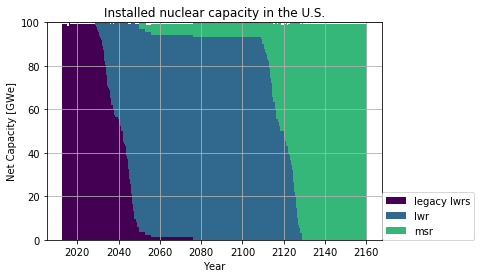
\includegraphics[scale=0.7]{./images/us/power_plot.png}
	\end{center}
	\caption{Power capacity separated by reactor type from 2020.}
	\label{fig:us_pow}
\end{figure}

\begin{figure}[htbp!]
	\begin{center}
		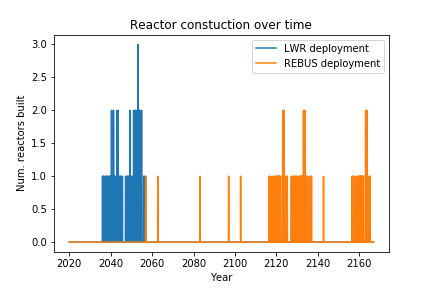
\includegraphics[scale=0.7]{./images/us/us_dep.png}
	\end{center}
	\caption{New reactor deployment from 2020.}
	\label{fig:us_dep}
\end{figure}

\section{Material flow}

The fuel cycle is represented by a series of facility agents whose material 
flow is illustrated in figure \ref{diag:us_fc}, along with
the \Cyclus archetypes that were used to model each facility.

\begin{figure}
	\centering
	\scalebox{0.6}{
		\begin{tikzpicture}[align=center, node distance = 3cm and 3cm, auto]
		% Place nodes
		\node [block] (sr) {Mine (\texttt{SOURCE})};
		\node [cloud, below of=sr] (nu) {Nat U};
		\node [block, below of=nu] (enr) {\small Enrichment ({\scriptsize \texttt{ENRICHMENT}})};
		\node [cloud, below of=enr] (uox) {\acrshort{UOX}};
		\node [block, below of=uox] (lwr) {\gls{LWR} (\texttt{REACTOR})};
		\node [cloud, right of=lwr] (snf) {\gls{UNF}};
		\node [block, right of=snf] (pool) {Pool (\texttt{Storage})};
		\node [cloud, left of=uox] (tl2) {Dep U};
		\node [block, below of=tl2] (stor) {Storage (\texttt{Storage})};
		\node [block, right of=tl] (sk) {Repository (\texttt{SINK})};
		\node [cloud, below of=sk] (cunf) {Cooled \gls{UNF}};
		\node [cloud, below of=pool] (cunf2) {Cooled \gls{UNF}};
		\node [block, below of=snf] (rep) {{\footnotesize Reprocessing ({\scriptsize \texttt{SEPARATIONS}})}};
		\node [cloud, below of=rep] (u) {Sep. U} ;
		\node [cloud, left of=rep] (pu) {Sep. TRU};
		\node [block, left of=pu] (mix) {Fabrication (\texttt{MIXER})};
		\node [cloud, below of=mix] (fs) {Fuel Salt};
		\node [block, below of=mox] (mxr) {\gls{MSR} (\small \texttt{SaltProc-} \\ \texttt{Reactor})};
		\node [cloud, left of=stor] (tl) {Dep U};
		
		\node [cloud, right of=mxr] (waste) {Waste};
		\node [cloud, below of=waste] (eols) {End-of-life salt};
		
		\draw[->, thick] (sr) -- (nu);
		\draw[->, thick] (nu) -- (enr);
		\draw[->, thick] (enr) -- (tl2);
		\draw[->, thick] (tl2) -- (stor);
		\draw[->, thick] (enr) -- (uox);
		\draw[->, thick] (uox) -- (lwr);
		\draw[->, thick] (lwr) -- (snf);
		
		\draw[->, thick] (lwr) -- (snf);
		\draw[->, thick] (snf) -- (pool);
		\draw[->, thick] (pool) -- (cunf);
		\draw[->, thick] (pool) -- (cunf2);
		\draw[->, thick] (cunf) -- (sk);
		\draw[->, thick] (cunf2) -- (rep);
		
		\draw[->, thick] (rep) -- (u);
		\draw[->, thick] (rep) -- (pu);
		\draw[->, thick] (pu) -- (mix);
		\draw[->, thick] (mix) -- (mox);
		\draw[->, thick] (mox) -- (mxr);
		
		\draw[->, thick] (stor) -- (tl);
		\draw[->, thick] (tl) to [bend right] (mxr);
		\draw[->, thick] (tl) -- (mix);
		\draw[->, thick] (nu) -- node{} ++ (-8cm, 0) |- (mix) ;
			
		\draw[->, thick] (mxr) -- (waste);
		\draw[->, thick] (waste) to [bend right=80] (sk);
		\draw[->, thick] (mxr) -- (eols);
		\draw[->, thick] (eols) to [bend right=80] (sk);		
		
		\end{tikzpicture}
		
	}
	\caption{Fuel cycle facilities (blue boxes) represented by 
		\Cyclus archetypes (in parentheses) pass materials (red 
		ovals) around the simulation.} 
	\label{diag:us_fc}
\end{figure}

The U.S. transition scenario's material flow is similar to that of the French transition
in the previous chapter,
except that all \gls{TRU} is reprocessed from \gls{LWR} \gls{UNF}
to fabricate fuel salt. Also, the depleted uranium from
the enrichment plant is stored in a storage facility to be used as a fertile stream for \gls{MSR} facilities.
Natural uranium is mixed with the reprocessed \gls{TRU} to create fuel salt.
Lastly, instead of a single
stream of \gls{MOX} \gls{UNF} from the \gls{MOX} reactors, \glspl{MSR}
output two streams - reprocess waste and end-of-life salt - which are both disposed.

\FloatBarrier


\section{Scenario specification}

The scenario specifications for the U.S. transition scenario are listed
in table \ref{tab:us_sim_specs}. The simulation end date is set to 2160
so that second generation of large \gls{MSR} deployment is included in the
simulation. \gls{MSR} fuel production begins 20 years prior to \gls{MSR}
deployment to reduce reprocessing and fabrication burden. \gls{LWR} \gls{UNF}
is cooled for a minimum of 8.5 years so that the \gls{TRU} vector is similar
to the \gls{TRU} vector of REBUS-3700 initial fuel (see figure \ref{fig:trutru}).
The reprocessing plant separates all \gls{TRU}, and mixes the separated \gls{TRU}
elements into \gls{MSR} fuel. 


\begin{table}[h]
	\centering
	\caption{Simulation Specifications}
	\begin{tabularx}{\linewidth}{bqq}
		\hline
		\textbf{Specification} &\textbf{ Value} & \textbf{Units}\\
		\hline
		Simulation Starts & 2013 & year\\
		Simulation Ends & 2160 & year\\
		Production of \gls{MSR} fuel begins & 2030 & year\\
		\glspl{MSR} become available & 2050 & year\\
		Reprocessed uranium usage &  None & -\\
		Minimum \gls{UNF} cooling time  & 8.5  & years\\
		Separation efficiency of \gls{TRU} and U & 99.8 & \% \\
		Reprocessing streams & Am, Pu, Cm, Np and U & - \\
		Reprocessing capacity & $\infty$ & \gls{MTHM}/month\\
		\gls{MSR} fuel salt fabrication throughput & No limit ($\infty$) & \gls{MTHM}/month \\
		\hline
	\end{tabularx}
	\label{tab:us_sim_specs}
\end{table}

\section{Reactor specifications}

Two major reactors are used in the simulation, \gls{PWR} and \gls{MSR}.
For \glspl{PWR}, I use a linear core size model to capture varying reactor capacity
(explained in section \ref{sec:writeinput}). The reactors deployed after 2020 are
modeled after the AP-1000 reactor \cite{sutharshan_ap1000tm_2011}, and I
assume a \gls{PWR} lifetime of 80 years. The reactor
specifications are shown in \ref{tab:us-reactor-specs}. The \gls{MSR} does not
have a refueling outage and runs continuously. 

\begin{table}[h]
	\centering
	\caption{Baseline \gls{LWR} and \gls{MSR} simulation specifications.}
	\begin{tabular}{lrr}
		\hline
		\textbf{Specification} & \textbf{\gls{PWR} \cite{sutharshan_ap1000tm_2011}} & \textbf{\gls{MSR} \cite{mourogov_potentialities_2006}} \\
		\hline
		Lifetime [y]  & 80 & 40 \\
		Cycle Time [mos.]& 18 & continuous \\ 
		Refueling Outage [mos.]& 2 & N/A \\
		Rated Power [\gls{MWe}] & 1110 & 1628 \\
		Assembly mass [kg] & 446 & N/A \\
		Batch mass [kg] & 23,192 & N/A \\
		Core mass [kg] & 70,022 & 200,100 \\
		Discharge Burnup [GWd/tHM] & 51 & N/A \\
		Assemblies per core & 157  & N/A \\
		Batches per core & 3 & N/A \\
		Initial Fissile Loading [t] & 3.1  $^{235}$U & 19.13 \gls{TRU} \\
		Fuel & \gls{UOX} & \gls{TRU}-U Cl Salt \\
		\hline
	\end{tabular}
	\label{tab:us-reactor-specs}
\end{table}


\section{Material definitions}
Depletion calculations for the \gls{LWR} nuclear fuel are recipe-based, such 
that a fresh and used fuel recipe is calculated beforehand using ORIGEN (see table \ref{tab:comp}).
ORIGEN calculates buildup, decay, and processing of radioactive materials
\cite{parks_overview_1992}. This recipe has also been used for
repository performance modeling \cite{wilson_adoption_2009}.
For fresh \gls{LWR} fuel, I assume a fuel enrichment of 3.1\% U235.

For depletion calculations of \gls{MSR} fuel, I use SaltProc (section \ref{sec:saltproc})
to obtain depleted fuel compositions and waste stream composition in a continuously
reprocessing reactor. The initial composition used in this simulation for the REBUS-3700
reactor is shown in table \ref{tab:rebus_init}.


\begin{table}[h]
	\centering
	\caption{Initial fuel salt composition for REBUS-3700}
	\begin{tabular}{lS}
		\hline
		\textbf{Isotope} & \textbf{Mass \%}\\
		\hline
		Na23	&	6.752	\\
		Cl35	&	26.753	\\
		Cl37	&	9.227	\\
		U235	&	0.343	\\
		U238	&	47.362	\\
		Np237	&	0.459	\\
		Pu238	&	0.204	\\
		Pu239	&	4.623	\\
		Pu240	&	2.12	\\
		Pu241	&	0.866	\\
		Pu242	&	0.61	\\
		Am241	&	0.494	\\
		Am243	&	0.142	\\
		Cm244	&	0.041	\\
		Cm245	&	0.004	\\
		\hline
	\end{tabular}
	
	\label{tab:rebus_init}
	
\end{table}

\section{Database generation}
The database used to model \glspl{MSR} is generated using SaltProc
with a unit cell model of the REBUS-3700 reactor. The parameters
used for running SERPENT and SaltProc are shown in table \ref{tab:saltproc-run-params}.
The parameters were chosen to acquire a reasonably accurate simulation result
while keeping the simulation time under 48 hours. I chose SERPENT simulation parameters
so that the eigenvalue ($k_{eff}$) uncertainties for any SERPENT run does not
exceed 42 ppm. The fuel salt density and power density was obtained from
values in the literature \cite{mourogov_potentialities_2006}. I derived
the fuel salt mass by dividing the core fuel mass by the core volume.
\[\rho_{fuel} = \frac{M_{core}}{V_{core}} = \frac{133.3 t}{368,587 l} = 3.6 \frac{g}{cm^3} \]
I set SaltProc simulation parameters to keep the number of SERPENT
3-day depletion calculations under 800.

\begin{table}[h]
	\centering
	\caption{SaltProc simulation parameters used to generate the database for REBUS-3700}
	\begin{tabular}{lr}
		\hline
		\textbf{Parameter} & \textbf{Value}\\
		\hline
		\multicolumn{2}{c}{\textbf{SERPENT Parameters}} \\
		\hline
		Num. neutrons per generation & 8,000 \\
		Num. active generation & 150\\
		Num. inactive generation & 50 \\
		Burnup calc. mode & CRAM \\
		Power density & $32.18e-3$ $\frac{kW}{g}$ \\ 
		Depletion step & 30 days\\
		Fuel salt density & $3.6 \frac{g}{cm^3}$ \\
		\hline
		\multicolumn{2}{c}{\textbf{SaltProc Parameters}} \\
		\hline
		Lifetime [y]  & 60 \\
		Total timesteps & 730 \\
		Reprocessing Scheme & As table \ref{tab:rebus_reproc}\\
		Refill material & Depleted uranium ($0.3\%$ $^{235}U$) \\
		\hline
	\end{tabular}
	\label{tab:saltproc-run-params}
\end{table}

The change in $K_{eff}$ values in the REBUS-3700 core during its lifetime is shown in figure \ref{fig:keff}.
A lifetime of 40 years is set for the REBUS-3700 reactor since the $k_{eff}$
value drops below 1.01 after 40 years of operation, according to the SaltProc results.
The REBUS reactor discharges
waste (reprocessed elements - in table \ref{tab:rebus_reproc}) at an average rate of
$90.34 \frac{kg}{month}$ (figure \ref{fig:rebus_waste}).


\begin{figure}[htbp!]
	\begin{center}
		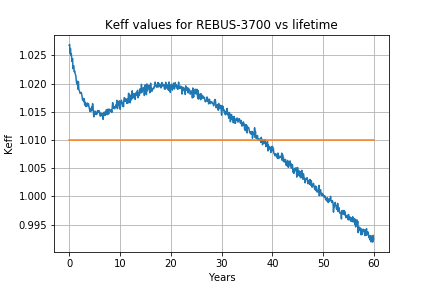
\includegraphics[scale=0.7]{./images/us/keff.png}
	\end{center}
	\caption{Change in $k_{eff}$ value in the REBUS-3700 core. The $k_{eff}$ drops below
		1.01 after 40 years of operation.}
	\label{fig:keff}
\end{figure}

\begin{figure}[htbp!]
	\begin{center}
		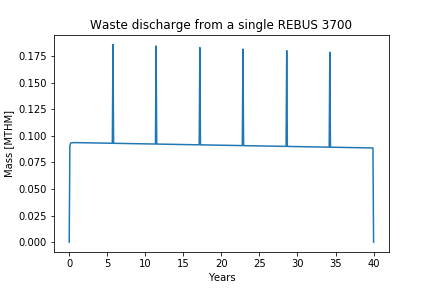
\includegraphics[scale=0.7]{./images/us/rebus_waste.png}
	\end{center}
	\caption{Mass of waste discharged from a single REBUS reactor. The peaks
		are due to the timestep differences in \Cyclus and SaltProc. \Cyclus
		uses 30.43 days for a month (1/12 of 365.25), and SaltProc uses 30-day
		timesteps. The peaks occur when two SaltProc timestep-worth of waste is discharged
		per one \Cyclus timestep.
	}
	\label{fig:rebus_waste}
\end{figure}

This database is generated to demonstrate \gls{MSR} modeling capability in \Cyclus,
and there is a possibility for future benchmarking if other simulation tools are
applied to the topic.


\FloatBarrier


\section{Results}
Results show that the United States can transition into a
fully \gls{MSR} fleet, while reducing final repository
burden by reducing \gls{TRU} and depleted uranium
inventory.

\subsection{LWR UNF inventory}

Table \ref{tab:us_lwr_unf} lists the U.S. \gls{LWR} \gls{UNF} inventory
results in the simulation.
Since major deployment of \glspl{MSR} does not begin until 2110,
the U.S. has a long time to prepare and accumulate the \glspl{TRU}
required for \gls{MSR} fuel salt fabrication. The U.S. accumulates
an additional $196,976$ \gls{MTHM} of \gls{LWR} \gls{UNF}
from 2013 to 2130, the year when the last \gls{LWR} decommissions.
Figure \ref{fig:us_lwr_unf} shows the accumulation of \gls{LWR} \gls{UNF}.
This figure does not subtract the \gls{LWR} \gls{UNF} reprocessed.


\begin{figure}[htbp!]
	\begin{center}
		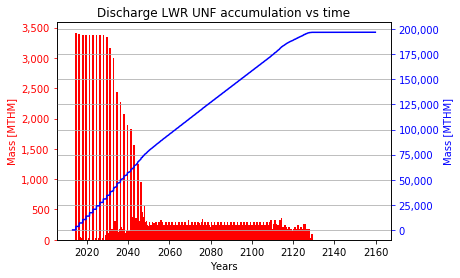
\includegraphics[scale=0.7]{./images/us/us_lwr_unf.png}
	\end{center}
	\caption{The cumulative mass of U.S. \gls{LWR} \gls{UNF}. The red bars are the
			mass discharged per timestep, and the blue line is the cumulative
			inventory. The large discharge quantity prior to 2040 is because the legacy \glspl{LWR}
			are deployed in the first timestep, thus discharging their fuel in sync.
			The later deployed \glspl{LWR} are not in sync, which makes the monthly
			discharge values more averaged out.}
	\label{fig:us_lwr_unf}
\end{figure}

\begin{table}[h]
	\centering
	\caption{U.S. \gls{LWR} \gls{UNF} material flow and inventory}
	\begin{tabular}{lrl}
		\hline
		\textbf{Category} & \textbf{Value [MTHM]} \\
		\hline
		US \gls{UNF} UOX generated in 2013-2050 & 78,281 \\
		US legacy \gls{LWR} \gls{UNF} in 2013 & 68,072 \\
		Total US \gls{LWR} \gls{UNF} inventory in 2050 & 146,353 \\
		Total US \gls{LWR} \gls{UNF} created from 2013 & 196,976 \\
		Total US \gls{LWR} \gls{UNF} created in U.S. & 265,048 \\
		\hline
	\end{tabular}
	\label{tab:us_lwr_unf}
\end{table}


\subsection{Reprocessing and fabrication material flow}

Metrics for \gls{LWR} \gls{UNF} reprocessing
are shown in table \ref{tab:us_rep}. A total of
$19,015$ MTHM of fuel salt is sent to \glspl{MSR}.
A total of $134,927$ MTHM of \gls{LWR} \gls{UNF}
are reprocessed to extract the \gls{TRU} for the fuel.

Figure \ref{fig:lwr_unf_reproc} shows the cumulative quantity of \gls{LWR}
\gls{UNF} reprocessed over time. The initial stage (2050-2100) is characterized
by a small amount of reprocessing due to the small number of \glspl{MSR} deployed.
From 2100, aggressive deployment of \glspl{MSR} causes
a large increase in the amount of \gls{LWR} \gls{UNF} reprocessed. This sudden
jump in demand of fuel salt is mediated by reprocessing the \gls{LWR} \gls{UNF} beforehand.

\begin{table}[h]
	\centering
	\caption{U.S. reprocessing metrics}
	\begin{tabular}{lS}
		\hline
		\textbf{Category} & \textbf{Value [MTHM]} \\
		\hline
		Total fuel salt mass sent to \gls{MSR}s & 19,015 \\
		Total TRU extracted from \gls{LWR} \gls{UNF} & 1,815 \\
		Total \gls{LWR} \gls{UNF} reprocessed & 134,927 \\
		Average monthly reprocessing demand of \gls{LWR} \gls{UNF} & 94.15 \\
		Average monthly fabrication of fuel salt & 13.26 \\
		Total raffinate stockpile & 4,024 \\
		\hline
	\end{tabular}
	\label{tab:us_rep}
\end{table}


\begin{figure}[htbp!]
	\begin{center}
		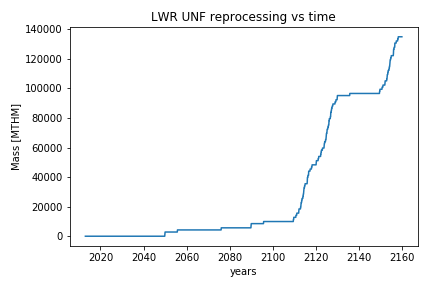
\includegraphics[scale=0.7]{./images/us/lwr_unf_reproc.png}
	\end{center}
	\caption{The Cumulative mass of \gls{LWR} \gls{UNF} reprocessed for \gls{MSR} salt fabrication.}
	\label{fig:lwr_unf_reproc}
\end{figure}

\subsection{Waste inventory and resource usage}

Table \ref{tab:us_waste} shows the masses of various nuclear waste
inventories at the end of the simulation. Large quantities of \gls{LWR}
\gls{UNF} ($132,094$ MTHM) and depleted uranium ($~1.1$ million tons)
remain unused, meaning that more \glspl{MSR} could have been deployed.
The tails usage from the \glspl{MSR} is not significant compared to
the quantity of tails accumulated ($~0.2\%$ of the total tails inventory).
One way to use more tails
is to substitute depleted uranium for initial
fuel salt fabrication. This would mean increasing the \gls{TRU} composition
in the fuel salt to make up for the decrease in $^{235}U$, which is viable,
since there are still $132,094$ MTHM of \gls{LWR} \gls{UNF} leftover
to extract \gls{TRU} from.

Figure \ref{fig:msr_waste} shows the monthly discharge and cumulative
inventory of waste from \glspl{MSR}. The discharge mass increases with
\gls{MSR} deployment. The mass of depleted uranium sent to \glspl{MSR} coincides
with the waste outflux, since the mass in the \gls{MSR} is kept constant.

\begin{table}[h]
	\centering
	\caption{U.S. waste metrics.}
	\begin{tabular}{lrl}
		\hline
		\textbf{Category} & \textbf{Value [MTHM]} \\
		\hline
			\gls{LWR} \gls{UNF} leftover inventory & 130,120 \\
			Total waste from \gls{MSR}s & 2,972 \\
			Total tails created from 2013 & 1,192,722 \\
			Total reprocessed uranium stockpile & 260,867 \\
			Total tails used & 2,972 \\
			Total remaining tails inventory & 1,189,753 \\
			Total natural U used & 1,389,698 \\
		\hline
	\end{tabular}
	\label{tab:us_waste}
\end{table}


\begin{figure}[htbp!]
	\begin{center}
		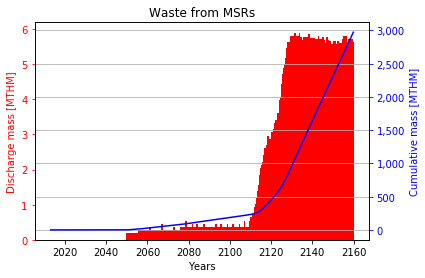
\includegraphics[scale=0.7]{./images/us/msr_waste.png}
	\end{center}
	\caption{Monthly discharged waste and cumulative waste inventory from
			\glspl{MSR}. The red bars are monthly discharge values, while
			the blue line is the cumulative quantity.}
	\label{fig:msr_waste}
\end{figure}


\section{Conclusion}
The United States can transition into a fully \gls{MSR} fleet with an
installed capacity of 100 GWe by 2130. With the deployment
scheme used in the simulation, the U.S. will have sufficient
time to prepare the fuel salt necessary for major \gls{MSR} deployment
beginning in 2110. Supporting the \gls{MSR} fleet requires an average
\gls{LWR} \gls{UNF} reprocessing capacity of $94.15$ MTHM per month, and an average fuel salt
fabrication capacity of $13.26$ MTHM per month. The reprocessing capacity demand is similar to the
current capacity of the La Hague plant in France (91.6 MTHM per month) \cite{schneider_spent_2008}.

The deployment of the REBUS-3700 \gls{MSR} design allows a reduction
in final repository burden, by transmuting the \gls{TRU} and reducing depleted uranium inventory.
However, \gls{TRU} extraction requires more advanced reprocessing methods than the currently
widely-deployed PUREX method. Resource utilization can be improved if depleted
uranium is used instead of natural uranium to fabricate initial fuel, since
there is still more than one million tons of depleted uranium available at the
end of the simulation. This would require a higher \gls{TRU} concentration
in the fuel, which is plausible since $132,094$ MTHM of \gls{LWR} \gls{UNF}
are still available for reprocessing.

In reality, however, complications with \gls{TRU} vectors and changes in \gls{MSR}
performance will occur, due to variations in \gls{LWR} \gls{UNF}
cooling (decay) time and discharge burnup. This would require careful fabrication of the initial fuel salt
so that the desired reactor parameters - multiplication factor, power density - are achieved. Another
challenge of this transition scenario is the aggressive build rates, which is not
considered in this work.

In conclusion, the U.S. can reduce its waste inventory by transitioning into
burner \glspl{MSR}. Choosing a U-Pu cycle instead of a Th-$^{233}U$ cycle
eliminates the need to introduce new resources (thorium), usage of moderators,
and allows utilization of depleted uranium, which would otherwise be waste.
Fissile (separated \gls{TRU}) and fertile (depleted uranium) material are
not limiting factors in the simulation, and a large inventory of \gls{LWR} \gls{UNF}
and depleted uranium remained at the end of the simulation.


\chapter{Conclusion and Future Work}
I simulated two different real-world nuclear fuel cycle transition scenarios,
where a \gls{LWR} fleet transitions into a \gls{FR} fleet with 
continuous plutonium and uranium reprocessing. Results show that important
parameters depend heavily on the initial condition of the simulation. France,
due to their long history of reprocessing \gls{LWR} \gls{UNF}, lacked the \gls{LWR}
\gls{UNF} inventory to readily transition to a \gls{SFR} fleet, thus requiring \gls{LWR}
\gls{UNF} from other \gls{EU} nations as well as a \gls{SFR} design with a high
breeding ratio. The U.S. on the other hand, started with a large \gls{LWR} \gls{UNF}
inventory of $68,071$ MTHM (~$7,000$ tons of plutonium), which allowed it the option of an aggressive nuclear capacity growth
and a low-breeding-ratio \gls{SFR} design.

This thesis demonstrates that fuel cycle analysis must be calculated with the real world initial conditions
in consideration, since the initial \gls{UNF} or plutonium inventory can have a large impact on what
nuclear reactor fuel cycle the nation can afford, or what reactor design to use to minimize
waste. In other words, a static, theoretical
fuel cycle analysis with no initial condition is inadequate for providing real-world insight.

This being said, for each fuel cycle analysis,
a central effort needs to be made on the knowledge of a nation's
initial conditions (current \gls{UNF} inventory and composition), its available
technologies (reactor technologies, fuel processing technologies), and the
projected energy demand.

\chapter{Appendix}

\appendix
\section{Fresh and Used Fuel Composition}
\begin{table}[h!]
        \centering
        \scalebox{0.45}{
                \begin{tabular}{cccc}
             Isotope     &      Used ASTRID Fuel &      Used UOX Fuel &         Used MOX Fuel \\
\hline
He4      &      8.2631E-05&     9.4745E-07 &    2.5108E-05 \\
Ra226    &      2.306EE-13&     9.7885E-14 &    6.8586E-14 \\
Ra228    &      6.029EE-21&     2.7508E-20 &    1.0769E-19 \\
Pb206    &      5.2269E-18&     5.5747E-18 &    3.6378E-18 \\
Pb207    &      1.0722E-15&     1.6859E-15 &    1.0589E-15 \\
Pb208    &      4.4347E-10&     3.6888E-12 &    2.0018E-12 \\
Pb210    &      1.3841E-16&     3.0238E-19 &    1.1829E-19 \\
Th228    &      7.7910E-10&     8.4756E-12 &    4.9017E-12 \\
Th229    &      3.5259E-11&     2.7278E-12 &    1.4379E-12 \\
Th230    &      1.1419E-08&     2.6258E-09 &    2.3998E-09 \\
Th232    &      6.3415E-11&     4.1748E-10 &    8.7655E-10 \\
Bi209    &      2.5042E-13&     6.6077E-16 &    2.6878E-16 \\
Ac227    &      2.8317E-14&     3.0968E-14 &    2.4608E-14 \\
Pa231    &      8.8076E-10&     9.2465E-10 &    7.0696E-10 \\
U232     &      1.4693E-07&     0.0000 &        5.9336E-10 \\
U233     &      4.0461E-08&     2.2139E-09 &    1.0359E-08 \\
U234     &      0.0010&         0.0001 &        0.0002 \\
U235     &      0.0003&         0.0076 &        0.0043 \\
U236     &      0.0005&         0.0057 &        0.0051 \\
U238     &      0.5864&         0.9208 &        0.8283 \\
Np237    &      0.0038&         0.0006 &        0.0043 \\
Pu238    &      0.0096&         0.0002 &        0.0060 \\
Pu239    &      0.0981&         0.0060 &        0.0410 \\
Pu240    &      0.0890&         0.0029 &        0.0283 \\
Pu241    &      0.0155&         0.0017 &        0.0146 \\
Pu242    &      0.0273&         0.0008 &        0.0098 \\
Pu244    &      1.779EE-07&     2.8648E-08 &    2.1888E-07 \\
Am241    &      0.0077&         6.4427E-05 &    0.0021 \\
Am242m   &      0.0005&         8.5336E-07 &    5.0357E-05 \\
Am243    &      0.0091&         0.0001 &        0.0020 \\
Cm242    &      0.0004&         2.5898E-05 &    0.0002 \\
Cm243    &      0.0000&         0.0000 &        1.2639E-05 \\
Cm244    &      0.0067&         8.5616E-05 &    0.0010 \\
Cm245    &      0.0017&         5.7217E-06 &    0.0001 \\
Cm246    &      0.0009&         7.2956E-07 &    6.1406E-06 \\
Cm247    &      0.0000&         0.0000 &        1.2059E-07 \\
Cm248    &      4.0265E-06&     7.6916E-10 &    9.1585E-09 \\
Cm250    &      1.076EE-12&     4.2808E-18 &    3.7338E-17 \\
Cf249    &      1.6590E-07&     1.6499E-12 &    4.0567E-11 \\
Cf250    &      9.5219E-09&     2.0419E-12 &    2.9328E-11 \\
Cf251    &      3.2032E-10&     9.8655E-13 &    1.4479E-11 \\
Cf 252   &      8.3754E-12&     6.5797E-13 &    7.5346E-12 \\
H3       &      3.1829E-07&     8.5846E-08 &    1.0269E-07 \\
Kr81     &      1.5156E-11&     4.2168E-11 &    7.3446E-11 \\
Kr85     &      0.0000&         3.4448E-05 &    2.0548E-05 \\
Sr90     &      0.0009&         0.0007 &        0.0004 \\
Tc99     &      0.0029&         0.0011 &        0.0011 \\
I129     &      0.0009&         0.0002 &        0.0003 \\
Cs134    &      0.0001&         0.0002 &        0.0002 \\
Cs135    &      0.0051&         0.0006 &        0.0009
                \end{tabular}}
                \caption{Spent Fuel Compositions}
                \label{tab:comp}
\end{table}




\bibliographystyle{unsrtnat}
\bibliography{bibliography}


\end{document}
\endinput
%%
%% End of file `thesis-ex.tex'.
